\section{Measure Spaces}

  Let's do a little refresher on measure theory. 

\subsection{Sigma Algebras and Measures}

  \begin{definition}[$\sigma$-algebra]
    A $\boldsymbol{\sigma}$\textbf{-algebra} on a set $X$ is a collection of subsets of $X$, denoted $\mathcal{A} \subset 2^X$, satisfying
    \begin{enumerate}
      \item Contains Empty Set: $\emptyset \in \mathcal{A}$ 
      \item Stability under Complementation: $A \in \mathcal{A} \implies A^c \in \mathcal{A}$, where $A^c = X - A$ 
      \item Stability under Countable Union: If $\{A_i\}$ is a countable sequence of sets, then 
      \begin{equation}
        \bigcup_i A_i \in \mathcal{A}
      \end{equation}
    \end{enumerate}
  \end{definition}

  At first, we might wonder why we need $\sigma$-algebras in the first place. We want to identify sets that are measurable in the way that their size can be determined, but why not just use $2^X$? This is because of the Banach-Tarski paradox, which gives you contradictions if you try to define a measure over $2^X$.  

  \begin{lemma}[Additional Property of $\sigma$-Algebras]
    A commonly known property of any $\sigma$-algebra $\mathcal{A}$ is that it is stable under countable intersections, too. 
    \begin{equation}
      A_1, A_2, \ldots, \in \mathcal{A} \implies \bigcap_{k=1}^\infty A_k \in \mathcal{A}
    \end{equation}
  \end{lemma}
  \begin{proof}
    We can utilize the fact that 
    \begin{equation}
      \bigcap_{k=1}^\infty A_k = X \setminus \bigcup_{k=1}^\infty A_k^c
    \end{equation}
  \end{proof}

  A $\sigma$-algebra is similar to the topology $\tau$ of topological space. Both $\mathcal{A}$ and $\tau$ require $\emptyset$ and $X$ to be in it. The three differences are that (i) $\tau$ does not allow compelmentation, (ii) $\tau$ allows any (even uncountable) union of sets (condition is strengthened), and (iii) $\tau$ allows only finite intersection of sets (condition is weakened). Now in order to construct $\sigma$-algebras, the following theorems are useful since they allow us to construct $\sigma$-algebras from other $\sigma$-algebras. It turns out that the intersection of $\sigma$-algebras is a $\sigma$-algebra, but not for unions. 

  \begin{theorem}
    Let $\{\mathcal{A}_k\}$ be a family of $\sigma$-algebras of $X$. Then, $\cap \mathcal{A}_k$ is also a $\sigma$-algebra of $X$. 
  \end{theorem}
  \begin{proof}
    Clearly, $\emptyset, X$ is in $\cap \mathcal{A}_k$. To prove complementation, 
    \begin{equation}
      A \in \bigcap \mathcal{A}_k \implies A \in \mathcal{A}_k \; \forall k \implies A^c \in A_k \; \forall k \implies A^c \in \bigcap \mathcal{A}_k
    \end{equation}
    To prove countable union, let $\{A_j\}_{j \in J}$ be some countable family of subsets in $\cap \mathcal{A}_k$. Then, 
    \begin{equation}
      A_j \in \bigcap \mathcal{A}_k \; \forall j \in J \implies A_j \in \mathcal{A}_k \; \forall k \forall j \implies \bigcup A_j \in \mathcal{A}_k \; \forall k \implies \bigcup A_j \in \bigcap \mathcal{A}_k
    \end{equation}
  \end{proof}

  This allows us to easily prove the following proposition, which just establishes the existence of $\sigma$-algebras. 

  \begin{proposition}
    Let $F \subset 2^X$ be a collection of subsets of $X$. Then there exists a unique smallest $\sigma$-algebra $\sigma(F)$ containing $F$. $\sigma(F)$ is called the $\sigma$-algebra \textbf{generated} by $F$. 
  \end{proposition}
  \begin{proof}
    Let us denote $\mathcal{M}$ as the set of all possible $\sigma$-algebras $\mathcal{B}$ of $X$. $\mathcal{M}$ is nonempty since it contains $2^X$. Then, the intersection 
    \begin{equation}
      \bigcap_{\mathcal{B} \in \mathcal{M}} \mathcal{B}
    \end{equation}
    is the unique smallest $\sigma$-algebra. 
  \end{proof}

  Now, how do we measure a size on subsets of $X$? We use measures. 

  \begin{definition}[Measure]
    Given a measurable space $(X, \mathcal{A})$, a \textbf{measure} is a function $\mu : \mathcal{A} \longrightarrow [0, +\infty]$ satisfying 
    \begin{enumerate}
      \item Positive Definite: $\mu(A) \geq \mu(\emptyset) = 0$ 
      \item Countable Additivity: For all countable collections $\{A_k\}_{k=1}^\infty$ of pairwise disjoint subsets $A_k \in \mathcal{A}$, 
      \begin{equation}
        \mu \bigg( \bigsqcup_{k=1}^\infty A_k \bigg) = \sum_{k=1}^\infty \mu(A_k)
      \end{equation}
      Remember that we are allowed to take countable unions inside our $\sigma$-algebra, so this makes sense. Disjointness is clearly important since if it wasn't, then $\mu(A) = \mu(A \cup A) = 2 \mu(A)$, which is absurd. 
    \end{enumerate}
    The triplet $(X, \mathcal{A}, \mu)$ is called a \textbf{measure space}. 
  \end{definition}

  \begin{theorem}[Properties of Measure]
    Let $\mu$ be a measure on $(X, \mathcal{A})$. 
    \begin{enumerate}
      \item Monotonicity: If $A \subset B$, then $\mu(A) \leq \mu(B)$. 
      \item Subadditivity: If $A \subset \cup_{i=1}^\infty A_i$, then $\mu(A) \leq \sum_{i=1}^\infty \mu (A_i)$ 
      \item Continuity from Above: If $A_1 \subset A_2 \subset A_3 \subset \ldots$, then 
      \begin{equation}
        \mu\bigg( \bigcup_{k=1}^\infty A_k \bigg) = \lim_{k \rightarrow \infty} \mu(A_k)
      \end{equation}
      \item Continuity from Below: If $A_1 \supset A_2 \supset A_3 \supset \ldots$ and $\mu(A_1) < \infty$, then 
      \begin{equation}
        \mu\bigg( \bigcap_{k=1}^\infty A_k \bigg) = \lim_{k \rightarrow \infty} \mu(A_k)
      \end{equation}
    \end{enumerate}
  \end{theorem}
  \begin{proof}
  Listed. 
  \begin{enumerate}
    \item Let $B \setminus A \coloneqq B \cap A^c$. Then, since $A$ and $B \setminus A$ are disjoint, we have 
    \begin{equation}
      \mu(B) = \mu\big( A \cup (B \setminus A) \big) = \mu(A) + \mu(B \setminus A) \geq \mu(A)
    \end{equation}
    
    \item We again try to divide this union into disjoint sets. Let $A_i^\prime = A \cap A_i$, and let $B_1 = A_1^\prime$ with 
    \begin{equation}
      B_i = A_i \setminus \bigcup_{j=1}^{i-1} A^\prime_j
    \end{equation}
    Since $B_i$'s are disjoint with $B_i \subset A_i$, we can use the first property to get 
    \begin{equation}
      \mu(A) = \sum_{i=1}^\infty \mu(B_i) \leq \sum_{i=1}^\infty \mu(A_i)
    \end{equation}
    
    \item This is the first time we introduce limits. With the fact that $\mu(A_k)$ must be nondecreasing, we can use real analysis and see that it is bounded by $\infty$, meaning that it must have a limit. But why does this limit equal to the left hand side? We can see that 
    \begin{align}
      \mu\bigg( \bigcup_{k=1}^\infty A_k \bigg) & = \mu(A_1) + \sum_{k=2}^\infty \mu(B_k) \\
      & = \mu(A_1) + \lim_{k \rightarrow \infty} \sum_{k=2}^\infty \mu(B_k) \\
      & = \lim_{k \rightarrow \infty} \mu(A_1 \cup B_2 \cup \ldots B_k)  = \lim_{k \rightarrow \infty} \mu(A_k) 
    \end{align}
    where $B_k = A_k \setminus A_{k-1}$. 
    
    \item The $\mu(A_1) < \infty$ is a necessary condition, since if we take $A_k = [k, \infty)$ on the real number line, then we have $\cap_{k=1}^\infty A_k = \emptyset$, but the limit of the measure is $\infty$. Well we can define $B_k = A_k \setminus A_{k+1}$ and write $\cap_{k=1}^\infty A_k = A_1 \setminus \cup_{k=1}^\infty B_k$, which means that 
    \begin{align}
      \mu\bigg( \bigcap_{k=1}^\infty A_k \bigg) & = \mu\bigg( A_1 \setminus \bigcup_{k=1}^\infty B_k \bigg) \\
      & = \mu(A_1) - \mu\bigg( \bigcup_{k=1}^\infty B_k\bigg) \\
      & = \mu(A_1) - \sum_{k=1}^\infty \mu(B_k) \\
      & = \mu(A_1) - \lim_{K \rightarrow \infty} \sum_{k=1}^K \mu(B_k) \\
      & = \lim_{K \rightarrow \infty} \bigg( \mu(A_1) - \sum_{k=1}^K \mu(B_k) \bigg) \\
      & = \lim_{K \rightarrow \infty} \mu \bigg( A_1 \setminus \bigcup_{k=1}^K B_k \bigg) = \lim_{K \rightarrow \infty} \mu(A_K)
    \end{align}
    Now the first line uses the fact that if $A \subset B$, then $\mu(B \setminus A) + \mu(A) = \mu(B)$, and with the further assumption that $\mu(A) < \infty$, we can subtract on both sides like we do with regular arithmetic. 
  \end{enumerate}
  \end{proof}

  \begin{theorem}[Inclusion Exclusion Principle]
    One familiar property commonly seen in probability and combinatorics is the inclusion exclusion principle. If $A, B \in \mathcal{A}$, 
    \begin{equation}
      \mu(A \cup B) = \mu(A) + \mu(B) - \mu(A \cap B)
    \end{equation}
    and by induction, if $A_1, \ldots, A_n \in \mathcal{F}$, then 
    \begin{equation}
      \mu\bigg( \bigcup_{i=1}^n A_i \bigg) = \sum_{i=1}^n \mu(A_i) - \sum_{i < j} \mu(A_i \cap A_j) + \sum_{i < j < k} \mu(A_i \cap A_j \cap A_k) + \ldots + (-1)^{n-1} \mu\bigg( \bigcap_{i=1}^n \mu(A_i) \bigg)
    \end{equation}
  \end{theorem}

  Finally, here is a definition which will be useful shortly when talking about how $\sigma$-algebras model knowledge. 

  \begin{definition}[Sub-$\sigma$-Algebras]
    Given a $\sigma$-algebra $\mathcal{F}$, a \textbf{sub-$\boldsymbol{\sigma}$-algebra} of $\mathcal{F}$ is a $\sigma$-algebra $\mathcal{G}$ s.t. $\mathcal{G} \subset \mathcal{F}$. 
  \end{definition}

  This will allows us to compare $\sigma$-algebras by taking two $\sigma$-algebras $\mathcal{G}, \mathcal{H} \subset \mathcal{F}$, which $\mu$ is guaranteed to be defined on since it is defined over $\mathcal{F}$. 

  \subsubsection[Construction of Measure on Rn]{Construction of Measure on $\mathbb{R}^n$}

  Let $\mathbb{R}^n$ be the continuum and $\mathcal{R}^n$ be the \textbf{Borel $\boldsymbol{\sigma}$-algebra}, defined as the $\sigma$-algebra generated by the open sets of $\mathbb{R}^n$. 

  \begin{example}[Stieltjes Measure Function]
    Measures on $(\mathbb{R}, \mathcal{R})$ are defined by giving a \textbf{Stieltjes measure function} with the following properties: 
    \begin{enumerate}
      \item $F$ is nondecreasing 
      \item $F$ is right continuous: 
      \begin{equation}
        \lim_{y \downarrow x} F(y) = F(x)
      \end{equation}
    \end{enumerate}
  \end{example}

  \begin{theorem}
    Associated with each Stieltjes measure function $F$ there is a unique measure $\mu$ on $(\mathbb{R}, \mathcal{R})$ with 
    \begin{equation}
      \mu((a, b]) = F(b) - F(a)
    \end{equation}
    When $F(x) = x$, then the resulting measure is called the \textbf{Lebesgue measure}. 
  \end{theorem}

  This is quite a hard proof, but we outline the construction of this measure on $\mathbb{R}$. First, we would like to define a "nice" set of half-open half-closed intervals, which we show is a semialgebra $\mathcal{S}$. We can easily define a measure $\mu$ on this semialgebra. We can extend this semialgebra to an algebra $\overline{\mathcal{S}}$, along with a proper extension $\overline{\mu}$ that is a unique measure on $\overline{\mathcal{S}}$. 

  \begin{definition}[Semialgebra, Algebra]
    A collection $\mathcal{S}$ of sets is said to be a \textbf{semialgebra} if 
    \begin{enumerate}
      \item it is closed under intersection 
      \item If $S \in \mathcal{S}$, then $S^c$ is a finite disjoint union of sets in $\mathcal{S}$
    \end{enumerate}
    A collection $\mathcal{A}$ of subsets is said to be an \textbf{algebra} if 
    \begin{enumerate}
      \item it is closed under union 
      \item it is closed under complementation
      \item the first two imply that it is closed under intersection
    \end{enumerate}
    We can see that a set that is a $\sigma$-algebra $\implies$ it is an algebra. 
  \end{definition}

  Here is an example of a semialgebra, which we will utilize in building a measure on $\mathbb{R}^n$.  

  \begin{example}
    Let $\mathcal{S}_d$ be the empty set plus all sets of the form 
    \begin{equation}
      (a_1, b_1] \times \ldots \times (a_d, b_d] \subset \mathbb{R}^d
    \end{equation}
    where $-\infty \leq a_i < b_i \leq +\infty$. $\mathcal{S}_d$ is a semialgebra since 
    \begin{equation}
      \bigg( \prod_i (a_i^1 , b_i^1] \bigg) \cap \bigg( \prod_i (a_i^2, b_i^2] \bigg) = \prod_i (\max\{a_i^1, a_i^2\}, \min\{b_i^1, b_i^2\}]
    \end{equation}
    and ...
  \end{example}

  Now, we show that we can extend this semialgebra to an algebra. 

  \begin{lemma}
    If $\mathcal{S}$ is a semialgebra, then $\overline{\mathcal{S}} = \{\text{finite disjoint unions of sets in } \mathcal{S}\}$ is an algebra, called the algebra generated by $\mathcal{S}$. 
  \end{lemma}
  \begin{proof}

  \end{proof}

  \begin{example}
    Given $\mathbb{R}$ and its semialgebra $\mathcal{S}_1$, then $\overline{\mathcal{S}}_1$ consists of the empty set and all sets of the form 
    \begin{equation}
      \bigcup_{i=1}^n (a_i, b_i] \text{ where } -\infty \leq a_i < b_i \leq +\infty
    \end{equation}
  \end{example}

  Now as for extending our measure function to $\overline{\mathcal{S}}$, we can simply use the properties. Note that since since an algebra is constructed from finite disjoint unions of a semialgebra, given that the finite collection $\{A_i\}_{i=1}^n$ all reside in $\mathcal{S}$ and are disjoint, then their disjoint union must be in $\overline{\mathcal{S}}$ and must be measurable, defined as 
  \begin{equation}
    \overline{\mu} \bigg( \bigsqcup_{i=1}^n A_i \bigg) = \sum_{i=1}^n \mu(A_i)
  \end{equation}

  \begin{definition}[$\sigma$-finite measure]
    Given a measure on an algebra $\mathcal{A}$, $\mu$ is said to be \textbf{$\boldsymbol{\sigma}$-finite} if there is a sequence of sets $A_1, A_2, \ldots \in \mathcal{A}$ s.t. $\mu(A_i) < \infty$ and $\cup_i A_i = \Omega$ . 
  \end{definition}

  \begin{theorem}
    Let $\mathcal{S}$ be a semialgebra and let $\mu$ defined on $\mathcal{S}$ have $\mu(\emptyset) = 0$. Suppose 
    \begin{enumerate}
      \item if $S \in \mathcal{S}$ is a finite disjoint union of sets $\{S_i\}_{i=1}^n$, then 
      \begin{equation}
        \mu(S) = \sum_{i=1}^n \mu(S_i)
      \end{equation}
      \item f $S$ is a countably infinite disjoint union of sets $\{S_j\}_{j=1}^\infty$, then 
      \begin{equation}
        \mu(S) \leq \sum_{j=1}^\infty \mu(S_j)
      \end{equation}
    \end{enumerate}
    Then, $\mu$ has a unique extension $\bar{\mu}$ that is a measure on $\overline{\mathcal{S}}$, the algebra generated by $\mathcal{S}$. If $\bar{\mu}$ is $\sigma$-finite, then there is a unique extension $\nu$ that is a measure on $\sigma(\mathcal{S})$ (the smallest $\sigma$-algebra containing $\mathcal{S}$). 
  \end{theorem}

\subsection{Probability Spaces}

  \begin{definition}[Probability Space]
    A \textbf{probability space} is a measure space $(\Omega, \mathcal{F}, \mathbb{P})$ with $\mathbb{P}(\Omega) = 1$. 
    \begin{enumerate}
      \item $\Omega$ is called the \textbf{sample space} and an element $\omega \in \Omega$ is called an outcome. 
      \item $\mathcal{F}$ is called the \textbf{event space} and an element $A \in \mathcal{F}$ is called an event. 
      \item The measure of an event $\mathbb{P}(A)$ is called the \textbf{probability} of that event. 
    \end{enumerate}
    We can think of the sample space $\Omega$ as the set of all conceivable futures and an event $F \in \mathcal{F}$ as some subset of conceivable futures. The probability $\mathbb{P}(F)$ represents our degree of certainty that our future will be contained in such an event. If some measure space $X$ has a finite total measure, we can construct a probability space from it by normalizing the measure. 
  \end{definition}

  \subsubsection{Sigma-Algebras as Models of Knowledge}

    Let us focus on the $\sigma$-algebra $\mathcal{F}$. We can see that the $\sigma$-algebra \textit{models our knowledge of the experiment}. That is, given some outcome space $\Omega$, let us have two $\sigma$-algebras $\mathcal{F}$ and $\mathcal{G}$ such that $\mathcal{F} \subset \mathcal{G}$, i.e. $\mathcal{F}$ is a sub-$\sigma$-algebra of $\mathcal{G}$. What does this mean? Remember that the elements of the event space are the events that can be measured. If $\mathcal{G}$ is \textit{finer} than $\mathcal{F}$, then every set $F$ that is $\mathcal{F}$-measurable is also $\mathcal{G}$-measurable, and so someone who has knowledge of $\mu$ over $\mathcal{G}$ knows more than another who has knowledge of $\mu$ over $\mathcal{F}$. 

    For example, let us have a dice roll, with $\Omega = \{1, 2, 3, 4, 5, 6\}$.
    \begin{enumerate}
      \item Abby's knowledge is modeled by $\mathcal{F} = \{\emptyset, \{1, 2, 3\}, \{4, 5, 6\}, \Omega\}$, with 
      \begin{equation}
        \mathbb{P}(F) = \begin{cases} 
          0 & \text{ if } F = \emptyset \\
          1/2 & \text{ if } F = \{1, 2, 3\}, \{4, 5, 6\} \\ 
          1 & \text{ if } F = \Omega \end{cases}
      \end{equation}
      \item Bob's knowledge is modeled by $\mathcal{G} = 2^\Omega$ with the following values 
      \begin{equation}
        \mathbb{P}(\{1\}) = \mathbb{P}(\{2\}) = \mathbb{P}(\{3\}) = \mathbb{P}(\{4\}) = \mathbb{P}(\{5\}) = \mathbb{P}(\{6\}) = \frac{1}{6}
      \end{equation}
    \end{enumerate}
    We can see that $\mathcal{F} \subset \mathcal{G}$ and that Bob has more information than Abby since from the values of $\mathbb{P}$ over his $\sigma$-algebra, he can deduce that $\mathbb{P}(\{1, 2, 3\}) = \mathbb{P}(\{1\}) + \mathbb{P}(\{2\}) = \mathbb{P}(\{3\}) = 1/2$ (and likewise for $4, 5, 6$). All Abby knows is that the probability that the roll is $1, 2, 3$ is $1/2$, but in her view, the individual probabilities may not be uniformly $1/6$ at all (it could be $\mathbb{P}(\{1\}) = \mathbb{P}(\{2\}) = 0$ and $\mathbb{P}(\{3\}) = 1/2$, for example). More specifically, Bob has \textit{complete} information of the experiment since $\mathcal{G} = 2^\Omega$, so he knows the probability of every possible event. But no matter how little information one has about the experiment, \textit{everybody} will always know that the probability that \textit{any} outcome will happen is $1$ (hence $\mathbb{P}(\Omega) = 1$) and the probability that no outcome will happen is $0$ ($\mathbb{P}(\emptyset) = 0$), which is consistent with the definition of $\sigma$-algebras requiring to have $\emptyset$ and $\Omega$. Note that we can have two $\sigma$-algebras s.t. both model incomplete information and aren't strictly finer than one another, i.e. $\mathcal{F} \not\subset \mathcal{G}$ and $\mathcal{G} \not\subset \mathcal{F}$. 

    Note that given the same random experiment, we don't need to always have the same sample space or the same random variable. For example, let's have a coin toss. One could be interested in whether it lands heads or tails, which means $\Omega = \{0, 1\}$, but another could be interested in the number of times the coin flips midair, in which $\Omega = \mathbb{N}_0$. We could even be interested in the set of all trajectories of the coin, which would result in a huge space of all trajectories of the flip, or the velocity at which it lands on the table, which would lead to $\Omega = \mathbb{R}^+$. 

    Note that as you get more and more information, your $\sigma$-algebra can "grow" and get closer to something that models complete information. This means that given some $\sigma$-algebra $\mathcal{F}$ that models complete information, we can take a sequence of nondecreasing sub-$\sigma$-algebras of $\mathcal{F}$ 
    \begin{equation}
      \mathcal{F}_1 \subset \mathcal{F}_2 \subset \ldots \subset \mathcal{F}_i \subset \ldots
    \end{equation}
    such that $\mathcal{F}_i \subset \mathcal{F}$, which models our increasing knowledge of the experiment. 

    \begin{definition}[Filtration]
      Let $(\Omega, \mathcal{F}, \mathbb{P})$ be a probability space and $I$ be an index set with total order $\geq$ (usually, $\mathbb{N}, \mathbb{R}$). For every $i \in I$, let $\mathcal{F}_i$ be a sub-$\sigma$-algebra of $\mathcal{F}$ satisfying 
      \begin{equation}
        \mathcal{F}_i \subset \mathcal{F}_j \text{ if } i \geq j
      \end{equation}
      Note that we do not write it as a sequence like before since $I$ may be uncountable. Then, a \textbf{filtration} $\mathbb{F} = \{\mathcal{F}_i\}_{i \in I}$ is a family of $\sigma$-algebras that are ordered nondecreasingly. If $\mathcal{F}$ is a filtration, then $(\Omega, \mathcal{F}, \mathbb{F}, \mathbb{P})$ is called a \textbf{filtered probability space}. 
    \end{definition}

    \begin{example}[Filtration of 3 Coin Tosses]
      Let us describe a concrete example of a 3-coin toss filtration. The probability space is 
      \begin{equation}
        \Omega = \{000, 001, 010, 011, 100, 101, 110, 111\}
      \end{equation}
      which has $8$ outcomes so a complete $\sigma$-algebra would consist of $2^8 = 256$ outcomes. 
      \begin{enumerate}
        \item Before the experiment, we have no information at all, so 
        \begin{equation}
          \mathcal{F}_0 = \{\emptyset, \Omega\}
        \end{equation}
        which has $2^{2^0} = 2$ elements. 
        
        \item After the first coin toss, we would have information on what the first flip landed on (whether it was of form $( 0, \ast, \ast)$ or $(1, \ast, \ast)$), so we have a $\sigma$-algebra generated by these two events 
        \begin{align*}
          \mathcal{F}_1 & = \sigma(\{( 0, \ast, \ast)\}, \{(1, \ast, \ast)\}) \\
          & = \sigma(\{000, 001, 010, 011\}, \{100, 101, 110, 111\}) \\
          & = \{\emptyset, \{000, 001, 010, 011\}, \{100, 101, 110, 111\}, \Omega\}
        \end{align*}
        which has $2^{2^1} = 4$ elements. 
        
        \item After the second coin toss, we would have information on what the first two flips landed on (whether it was of form $( 0, 0, \ast)$, $( 0, 1, \ast)$, $(1, 0, \ast)$, $(1, 1, \ast)$), so we have a $\sigma$-algebra generated by these 4 events 
        \begin{align}
          \mathcal{F}_2 & = \sigma(\{( 0, 0, \ast)\}, \{( 0, 1, \ast)\}, \{(1, 0, \ast)\}, \{(1, 1, \ast)\}) \\
          & = \sigma(\{000, 001\}, \{010, 011\}, \{100, 101\}, \{110, 111\}) \\
          & = \{\emptyset, \{000, 001\}, \{010, 011\}, \{100, 101\}, \{110, 111\}, \\
          & \;\;\;\;\;\; \{000, 001, 010, 011\}, \{000, 001, 100, 101\}, \{000, 001, 110, 111\}, \\
          & \;\;\;\;\;\; \{010, 011, 100, 101\}, \{010, 011, 110, 111\}, \{100, 101, 110, 111\}, \\ 
          & \;\;\;\;\;\; \{000, 001, 010, 011, 100, 101\}, \{000, 001, 010, 011, 110, 111\}, \\
          & \;\;\;\;\;\; \{000, 001, 110, 101, 110, 111\}, \{010, 011, 110, 101, 110, 111\},  \Omega\}
        \end{align}
        which has $2^{2^2} = 16$ elements. 
        
        \item After the third coin toss, we would have information on what the first three flips landed on (all 8 possibilities in $\Omega$), so we have a $\sigma$-algebra generated by these 8 events 
        \begin{align}
          \mathcal{F}_3 & = \sigma(\{000\}, \{001\}, \{010\}, \{011\}, \{100\}, \{101\}, \{110\}, \{111\})
        \end{align}
        This is too big to write down explicitly, but it has $2^{2^3} = 256$ elements. 
      \end{enumerate}
    \end{example}

  \subsubsection{Types of Probability Spaces}

    \begin{definition}[Discrete Probability Space]
      If $\Omega$ is a countable set, then we can take its $\sigma$-algebra $\mathcal{F}$ to be the power set of $\Omega$ and construct the measurable space $(\Omega, 2^\Omega, \mathbb{P})$. From the axioms, for any event $A \in \mathcal{F}$, we have
      \begin{equation}
        \mathbb{P} (A) = \sum_{\omega \in A} \mathbb{P}(\{\omega\}) \text{ and } \sum_{\omega \in \Omega} \mathbb{P}(\{\omega\}) = 1
      \end{equation}
      The greatest $\sigma$-algebra $F = 2^{\Omega}$ describes the complete information. The cases $\mathbb{P}(\{\omega\}) = 0$ is permitted by the definition, but rarely used since such $\omega$ can safely be excluded from the sample space. Therefore, we can define the probability measure $\mathbb{P}$ by simply defining it for all singleton sets $\{\omega\}$. 
    \end{definition}

    This may be confusing, since for discrete spaces, it looks like we're assigning probabilities to each $\omega \in \Omega$, but we are actually assigning them to singleton \textit{sets}. We should be writing $\mathbb{P}(\{\omega\})$, but sometimes we abuse notation and write $\mathbb{P}(\omega)$. 

    \begin{example}
      Consider the flip of a fair coin with outcomes either hands or tails. Then, $\Omega = \{H, T\}$. The $\sigma$-algebra $F = 2^{\Omega}$ contains $2^2 = 4$ events: 
      \begin{align*}
        \{\} &= \text{Neither heads nor tails} \\
        \{H\} &= \text{Heads} \\
        \{T\} &= \text{Tails} \\
        \{H, T\} &= \text{Either heads or tails}
      \end{align*}
      That is, $\mathcal{F} = \{\{\}, \{H\}, \{T\}, \{H, T\}\}$. Our probability measure $\mathbb{P}$ is defined
      \begin{equation}
        \mathbb{P}(f) = \begin{cases}
        0 & f = \{\} \\
        0.5 & f = \{H\} \\
        0.5 & f = \{T\} \\
        1 & f = \{H, T\}
        \end{cases}
      \end{equation}
    \end{example}

    Being able to consider the event space as $2^X$ is very nice, since countability of $X$ allows us to avoid the Banach-Tarski paradox. It doesn't matter whether $\mathcal{F} = 2^X$ itself is uncountable or not. 

    \begin{example}[3 Coin Tosses]
      A fair coin is tossed 3 times, creating 8 possible outcomes. 
      \begin{equation}
        \Omega = \{HHH, HHT, HTH, HTT, THH, THT, TTH, TTT\}
      \end{equation}
      The complete information is described by the $\sigma$-algebra $\mathcal{F} = 2^{\Omega} = 2^8 = 256$ events, where each of the events is a subset of $\Omega$. 

      Alice knows the outcome of the second toss only. Thus, her incomplete information is described by the partition 
      \begin{equation}
        \Omega = A_1 \sqcup A_2 = \{HHH, HHT, THH, THT\} \sqcup \{HTH, HTT, TTH, TTT\}
      \end{equation}
      and the corresponding $\sigma$-algebra is 
      \begin{equation}
      \mathcal{F}_{Alice} = \{\emptyset, A_1, A_2, \Sigma\}
      \end{equation}
      Bryan knows only the total number of tails, so his partition contains 4 parts: 
      \begin{align*}
        \Omega & = B_0 \sqcup B_1 \sqcup B_2 \sqcup B_3 \\
          & = \{HHH\} \sqcup \{HHT, HTH, TTH\} \sqcup \{TTH, THT, HTT\} \sqcup \{TTT\}
      \end{align*}
      When we calculate Bryan's event space, we have
      \begin{align*}
        \mathcal{F}_{Bryan} & = \big\{\emptyset, \{HHH\}, \{HHT\}, \{HTH\}, \{THH\}, \{HHT, HTH\}, \{HHT, THH\}, \\
        & \;\;\;\;\{TTH, THT\}, \{TTH\}, \{THT\}, \{HTT\}, \{TTH, THT\},\{TTH, HTT\}, \\
        & \;\;\;\;\{THT, HTT\}, \{TTT\}, \Omega \big\} 
      \end{align*}
      Note that the event space of Bryan (and Alice) is not merely just $2^{\Omega}$ since we have some predetermined knowledge of the outcome space $\Omega$. Therefore, we can partition it into 4 cases and construct the event space by putting only the events that are subsets of each partition. For example, it wouldn't make sense to have an event 
      \begin{equation}
        \{HHH, TTT\}
      \end{equation}
      since the events $\{HHH\}$ and $\{TTT\}$ are in completely different outcome spaces (given the number of tails). That is, if we knew that 3 tails were thrown, the event $\{HHH, TTT\}$ wouldn't make any sense. However, the event $\Omega$ or $\emptyset$ is viable since they describe the case of whether the coin was tossed at all or not. 
      Furthermore, $\mathcal{F}_{Alice}$ and $\mathcal{F}_{Bryan}$ are incomparable. That is, $\mathcal{F}_{Alice} \not\subseteq \mathcal{F}_{Bryan}$ and $\mathcal{F}_{Bryan} \not\subseteq \mathcal{F}_{Alice}$, even though both are subalgebras of $2^{\Omega}$. 
    \end{example}

    \begin{example}[Geometric Measure on $\mathbb{N}$]
      Let $\Omega = \mathbb{N}$ and $\mathcal{F} = 2^\mathbb{N}$. We can completely define the probability measure by assigning them to singletons $k \in \mathbb{N}$. One such assignment is 
      \begin{equation}
        \mathbb{P}(\{k\}) = \frac{1}{2^k}
      \end{equation}
      or more generally, 
      \begin{equation}
        \mathbb{P}(\{k\}) = p (1 - p)^{k-1}
      \end{equation}
    \end{example}

    \begin{example}[Poisson Measure on $\mathbb{N}_0$]
      Let $\Omega = \mathbb{N} \cup \{0\}$. Then, $\mathcal{F} = 2^\Omega$ and we can define $\mathbb{P}$ on the singleton sets as 
      \begin{equation}
        \mathbb{P}(\{k\}) = \frac{e^{-\lambda} \lambda^k}{k!}
      \end{equation}
      for any $\lambda > 0$. We can then compute the probability of, say all primes, by taking 
      \begin{equation}
        \mathbb{P}(\text{primes}) = \sum_{k \text{ prime}} \mathbb{P}(\{k\})
      \end{equation}
      which we know to be monotonically increasing and bounded above, so it must converge. Whether this has a closed form solution is another matter. Again, in reality we are assigning probability measures on all $\mathcal{F}$-measurable sets, but just doing it through assignment of measure through singleton sets. 
    \end{example}
    
    \begin{example}[Voters]
      If $100$ voters are to be drawn randomly from among all voters in California and asked whom they will vote for governor, then the set of all sequences of $100$ Californian voters would be the sample space $\Omega$. We assume that sampling without replacement is used: only sequences of $100$ different voters are allowed. For simplicity an ordered sample is considered, that is a sequence $\{Alice, Bryan\}$ is different from $\{Bryan, Alice\}$. We also take for granted that each potential voter knows exactly his/her future choice, that is he/she doesn’t choose randomly.

      Alice knows only whether or not Arnold Schwarzenegger has received at least $60$ votes. Her incomplete information is described by the $\sigma$-algebra $\mathcal{F}_{Alice}$ that contains:
      \begin{enumerate}
        \item the set of all sequences in $\Omega$ where at least $60$ people vote for Schwarzenegger
        \item the set of all sequences where fewer than $60$ vote for Schwarzenegger
        \item the whole sample space $\Omega$
        \item the empty set $\emptyset$
      \end{enumerate}
      Bryan knows the exact number of voters who are going to vote for Schwarzenegger. His incomplete information is described by the corresponding partition $\Omega = B_0 \sqcup B_1 \ldots B_{100}$ and the $\sigma$-algebra $\mathcal{F}_{Bryan}$ consists of $2^{101}$ events. 

      In this case Alice’s $\sigma$-algebra is a subset of Bryan’s: $\mathcal{F}_{Alice} \subset \mathcal{F}_{Bryan}$. Bryan’s $\sigma$-algebra is in turn a subset of the much larger "complete information" $\sigma$-algebra $2^{\Omega}$ consisting of $2^{n(n-1)\ldots (n-99)}$ events, where $n$ is the number of all potential voters in California. 
    \end{example}

    Now if we move to uncountable outcome spaces, then things are not as nice, which is why we need to machinery of measure theory to study them. Let us try to model a probability measure on $\Omega = [0, 1]$. It is uncountable, and it turns out that $2^\Omega$ has cardinality strictly greater than even the continuum. If we try to model a uniform probability measure $\mathbb{P}$, then for some subset $A \in 2^\Omega$, it should be the case that $\mathbb{P}(A) = \mathbb{P}(A \oplus k)$, where $A \oplus k$ is just some translated version of $A$ still contained within $[0, 1]$. This applies to singleton sets, and it turns out that if we try to assign a nonzero probability measure to any singleton $\{k\}$, then the probability measure of $\Omega$ blows up to infinity, which we can't have. So the only thing we can do is have every singleton have zero probability. Remember that a measure by definition has the \textit{countable additivity} property, which says that 
    \begin{equation}
      \mu \bigg( \bigsqcup_{k=1}^\infty A_k \bigg) = \sum_{k=1}^\infty \mu(A_k)
    \end{equation}
    for all \textit{countable} collections $\{A_k\}$. Summation is not defined for uncountable collections, and so having a probability $0$ on every singleton does not imply that the probability of any uncountable set has is $0$. That is, having $\mathbb{P}(\{k\}) = 0$ for all $k \in [0, 1]$ does not tell you what $\mathbb{P}([0, 1])$ is. So now rather than assigning probabilities to singletons, like we did with discrete sets, the approach is to assign probabilities directly to our event space $\mathcal{F}$. We can do this by directly assigning the Lebesgue measure to the Borel algebra of $[0, 1]$, which has the properties 
    \begin{enumerate}
      \item $\mathbb{P}((a, b)) = \mathbb{P}([a, b)) = \mathbb{P}((a, b]) = \mathbb{P}([a, b]) = b - a$
      \item Translation invariance as stated above. 
    \end{enumerate}
    Over uncountable $\Omega$, we cannot afford to work with $2^\Omega$, since there is an impossibility theorem that says that there is no measure defined on $2^{[0, 1]}$ with the two properties above. Therefore, we must work with a smaller $\sigma$-algebra. Since the subsets of interest are usually intervals (or more generally, open sets), people usually take the Borel $\sigma$-algebra of open intervals on $[0, 1]$. The Lebesgue measure on $\mathbb{R}$ is not a probability measure since it $\lambda(\mathbb{R}) = \infty$, but we can construct a uniform probability measure on any bounded set of $\mathbb{R}$. Usually, these continuous probability spaces are $\mathbb{R}^n$, and we define some measure $\mu$ directly on its $\sigma$-algebra. 

    \begin{definition}[Atom]
      Let $(\Omega, \mathcal{F}, \mathbb{P})$ be uncountable. If for some $\omega \in \Omega$, $\mathbb{P}(\{\omega\}) \neq 0$, then $\omega$ is called an \textbf{atom}. 
    \end{definition}

    Now, given a general (discrete or continuous, or a combination of both) distribution, the set of all the atoms are an at most countable (maybe empty) set whose probability is the sum of probabilities of all atoms (by countable additivity). That is, given $\omega_1, \omega_2, \ldots$ atoms, 
    \begin{equation}
      \mathbb{P} \bigg( \bigsqcup_{i=1}^\infty \{\omega_i\} \bigg) = \sum_{i=1}^\infty \mathbb{P}(\{\omega_i\})
    \end{equation}
    \begin{enumerate}
      \item If this sum is equal to $1$ then all other points can be safely excluded from the sample space $\Omega$, returning us to the discrete case. 
      \item If this sum is $0$ then we just have some continuous sample space. This means $\mathbb{P}(\{\omega\}) = 0$ for all $\omega \in \Omega$, and so $\Omega$ must be uncountable (since if it was countable, then we should be able to sum the $\mathbb{P}(\{\omega\})$'s to get $1$, but it's $0$). Remember that summation is only defined for at most countable elements. 
      \item If the sum of probabilities of all atoms is strictly between $0$ and $1$, then the probability space decomposes into a discrete, atomic part and a non-atomic, continuous part. 
    \end{enumerate}

  \subsubsection{Conditioning on Events}

    \begin{definition}[Conditional Probability w.r.t. Events]
      Given a measure space $(\Omega, \mathcal{F}, \mathbb{P})$, let $B$ be an event such that $\mathbb{P}(B) > 0$. The \textbf{conditional probability} of $A$ given $B$ is defined 
      \begin{equation}
        \mathbb{P}(A \mid B) = \frac{\mathbb{P}(A \cap B)}{\mathbb{P}(B)}
      \end{equation}
    \end{definition}

    Note that we can't condition on events that have probability $0$, which is why we need the $\mathbb{P}(B) > 0$ condition. If this is the case, it doesn't even make sense to talk about a conditional probability $\mathbb{P}(A \mid B)$. For example, if we take the probability space $[0, 1]$ with its Borel algebra and the Lebesgue measure, then we cannot condition something on the rationals, e.g. $\mathbb{P}(\{\omega < 0.5\} \mid \omega \in \mathbb{Q})$ does not make sense. In fact, doing so can lead to contradictions, one being the \textbf{Borel-Kolmogorov paradox}. 

    An extremely useful theorem is that the conditional probability taken as a measure gives us a new viable measure on the same probability space $\Omega$. 

    \begin{theorem}
      Given probability space $(\Omega, \mathcal{F}, \mathbb{P})$, let $B \in \mathcal{F}$ with $\mathbb{P}(B) > 0$. Then, $\mathbb{P}( \cdot \mid B): \mathcal{F} \longrightarrow [0, 1]$ is a probability measure on $(\Omega, \mathcal{F})$. 
    \end{theorem}
    \begin{proof}
      We prove the properties of a probability measure. 
      \begin{enumerate}
        \item The empty set has measure $0$. 
        \begin{equation}
          \mathbb{P}(\emptyset \mid B) = \frac{\mathbb{P}( \emptyset \cap B)}{\mathbb{P}(B)} = \frac{\mathbb{P}(\emptyset)}{\mathbb{P}(B)} = \frac{0}{\mathbb{P}(B)} = 0
        \end{equation}
        \item The entire space has measure $1$. 
        \begin{equation}
          \mathbb{P}(\Omega \mid B) =  \frac{\mathbb{P}( \Omega \cap B)}{\mathbb{P}(B)} = \frac{\mathbb{P}(B)}{\mathbb{P}(B)} = 1
        \end{equation}
        \item Countable additivity of disjoint events. Let $A_i \in \mathcal{F}$ for $i = 1, 2, \ldots$ which are disjoint. Then, their union is in $\mathcal{F}$ by definition of $\sigma$-algebra. Now, 
        \begin{align*}
          \mathbb{P}\bigg( \bigcup_{i=1}^\infty A_i \bigg| B \bigg) & = \frac{1}{\mathbb{P}(B)} \mathbb{P} \bigg[ \Big( \bigcup_{i=1}^\infty A_i \Big) \cap B \bigg] \\
          & = \frac{1}{\mathbb{P}(B)} \mathbb{P} \bigg[ \bigcup_{i=1}^\infty (A_i \cap B) \bigg] \\
          & = \frac{1}{\mathbb{P}(B)} \sum_{i=1}^\infty \mathbb{P} (A_i \cap B) \\
          & = \sum_{i=1}^\infty \frac{\mathbb{P} (A_i \cap B)}{\mathbb{P}(B)} = \sum_{i=1}^\infty \mathbb{P}(A_i \mid B) 
        \end{align*}
      \end{enumerate}
    \end{proof}

    \begin{lemma}[Law of Total Probability]
      Suppose $A_1, A_2, ..., A_n$ is a partition of $\Omega$. Then, 
      \begin{equation}
        \{B \cap A_k\}_{k=1}^n
      \end{equation}
      is a partition of $B$, and 
      \begin{equation}
        \mathbb{P}(B) = \sum_{k=1}^n \mathbb{P} (B|A_k)\, \mathbb{P}(A_k)
      \end{equation}
      This is also called the \textit{Partition rule}. 
    \end{lemma}

    \begin{theorem}[Bayes Rule]
      Let $A, B \in \mathcal{F}$. Then, 
      \begin{equation}
        \mathbb{P}(B \mid A) = \frac{\mathbb{P}(A \mid B) \, \mathbb{P}(B)}{\mathbb{P}(A)}
      \end{equation}
    \end{theorem}
    \begin{proof}
      We know that 
      \begin{equation}
        \mathbb{P}(A \mid B) = \frac{\mathbb{P} (A \cap B)}{\mathbb{P}(B)} \text{ and } \mathbb{P}(B \mid A) = \frac{\mathbb{P}(B \cap A)}{\mathbb{P}(B)}
      \end{equation}
      and so we can write 
      \begin{equation}
        \mathbb{P} (A \mid B) \, \mathbb{P}(B) = \mathbb{P}(A \cap B) = \mathbb{P}(B \mid A) \, \mathbb{P}(A)
      \end{equation}
    \end{proof}

\subsection{Distributions, Random Variables, Measurable Functions}

  Random variables are motivated by the following. When you have a random experiment, the experimenter may not be interested in the specific elementary outcomes. So if you have sample space $\Omega$, you may not be concerned about what $\omega \in \Omega$ shows up, but more interested in some numerical function of the elementary outcome. For example, if you toss a coin 10 times, you're not interested in what sequence in $\{0, 1\}^{10}$ shows up, but you may want to just know how many heads came up. In other words, your interest defines a numerical function $X: \Omega \rightarrow \mathbb{R}$. This is useful, since in many cases the sample space $\Omega$ can be extremely complicated (e.g. the sample space of all weather conditions) and the elementary outcomes also complicated, so you may want to know some simpler aspect (e.g. the temperature). 

  The name "random variable" is very misleading. It's not random nor a variable. It is a deterministic function $X: (\Omega, \mathcal{F}, \mathbb{P}) \longrightarrow \mathbb{R}$ that assigns numbers to outcomes. The only source of randomness itself is which $\omega \in \Omega$ is chosen. But we can't just choose any function on $\Omega$; they must satisfy the nice property of measurability. Now, to talk about random variables, recall that the definition of a measurable function $f: (X, \mathcal{A}) \longrightarrow \mathbb{R}$ is one where the preimage of every Borel set $B \in \mathcal{R}$ is in $\mathcal{A}$. With a potential measure $\mu$, this allows us to define the Lebesgue integral of $f$. Note that this is also equivalent to the more easily provable fact that the preimage of every half-interval $(-\infty, t)$ is in $\mathcal{A}$. That is, $f^{-1}((-\infty, t]) \in \mathcal{A}$ for all $t \in \mathbb{R}$. 

  \begin{definition}[Random Variable]
    A \textbf{random variable} $X$ on probability space $(\Omega, \mathcal{F}, \mathbb{P})$ is an $\mathcal{F}$-measurable function $X: (\Omega, \mathcal{F}, \mathbb{P}) \longrightarrow \mathbb{R}$. That is, for every subset $B \in \mathcal{R}$, its preimage 
    \begin{equation}
      X^{-1} (B) = \{\omega \in \Omega \mid X(\omega) \in B\} \in \mathcal{F}
    \end{equation}
  \end{definition}

  The reason we want $X$ to be $\mathcal{F}$-measurable is because now we can define probabilities on Borel sets $B$ of $\mathbb{R}$ by computing the probabilities of the preimage of $B$, which must be $\mathcal{F}$-measurable. In a way, a random variable "pushes forward" the probability measure $\mathbb{P}$, originally defined on $\mathcal{F}$, to $\mathcal{R}$.  

  \begin{definition}[Probability Law of Random Variable $X$]
    Let $X$ be a random variable on probability space $(\Omega, \mathcal{F}, \mathbb{P})$. The \textbf{probability law of $X$} is a function $\mathbb{P}_X : \mathcal{R} \longrightarrow [0, 1]$ defined, for each Borel set $B$ of $\mathbb{R}$, as 
    \begin{equation}
      \mathbb{P}_X (B) \coloneqq \mathbb{P} \big( X^{-1}(B) \big) = \mathbb{P} \big( \{\omega \in \Omega \mid X(\omega) \in B\} \big)
    \end{equation}
    Note that $\mathbb{P}$ refers to the probability measure on $\mathcal{F}$, and $\mathbb{P}_X$ refers to the probability law on $\mathcal{R}$. In shorthand, we can write $\mathbb{P}_X = \mathbb{P} \circ X^{-1}$. By abuse of notation, it is generally written
    \begin{equation}
      \mathbb{P}(X \in B)
    \end{equation}
    It is important to get used to this notation. Whenever we write $\mathbb{P}(X \ldots)$, we are always working in the probability law of $X$. Furthermore, whatever condition we put within the parentheses describes a measurable set. For example, 
    \begin{enumerate}
      \item $\mathbb{P}(X = x)$ describes the probability law of $X$ evaluated on the set $\{x\}$. 
      \item $\mathbb{P}(X \leq x)$ describes the probability law of $X$ evaluated on the set $(-\infty, x]$. 
      \item $\mathbb{P}(Y \leq y)$ describes the probability law of $Y$ evaluated on the set $(-\infty, y]$.
      \item $\mathbb{P}(a \leq Y < b)$ describes the probability law of $Y$ evaluated on the set $[a, b)$. 
      \item $\mathbb{P}(Z \in \mathbb{Q})$ describes the probability law of $Z$ evaluated on the set $\mathbb{Q}$. 
    \end{enumerate}
  \end{definition}

  \begin{theorem}[$\sigma$-Algebra Generated by Random Variable $X$]
    Given probability space $(\Omega, \mathcal{F}, \mathbb{P})$ and a random variable $X$, $\mathbb{P}_X$ is a probability measure on $(\mathbb{R}, \mathcal{R})$. Now, it turns out that the collection of all preimages of Borel sets under $X$ forms a $\sigma$-algebra on $\Omega$. We call it 
    \begin{equation}
      \sigma(X) \coloneqq \big\{ A \subset \Omega \mid A = X^{-1}(B) \text{ for some } B \in \mathcal{R} \big\}
    \end{equation}
    which is a $\sigma$-algebra of $\Omega$. Since $X$ is a measurable function, every $X^{-1}(B)$ is $\mathcal{F}$-measurable, and so $\sigma(X)$ is a sub-$\sigma$-algebra of $\mathcal{F}$. It is never the case that $\sigma(X) \supset \mathcal{F}$, since that means that $X$ itself is not $\mathcal{F}$-measurable. 
  \end{theorem}

  \begin{theorem}
    Given $(\Omega, \mathcal{F}, \mathbb{P})$ and a random variable $X: \Omega \rightarrow \mathbb{R}$, let us define a probability law $\mathbb{P}_X = \mathbb{P} \circ X^{-1}$. Then, 
    \begin{equation}
      (\mathbb{R}, \mathcal{R}, \mathbb{P}_X)
    \end{equation}
    is a probability space. 
  \end{theorem}

  This theorem is extremely useful, since in practical applications, one does not consider an abstract $\Omega$ and works immediately in $\mathbb{R}$. Once we have determined our numerical values of interest (heads or tails, number of heads, sum of dice rolls) with our random variable $X$, we can just throw away $(\Omega, \mathcal{F}, \mathbb{P})$ and work directly in probability space $(\mathbb{R}, \mathcal{R}, \mathbb{P}_X)$. Therefore, we don't actually control $\Omega$ by explicitly defining it as we said before. 

  We could just leave $\Omega$ to be some arbitrary large set, and construct an appropriate random variable $X$ that will generate an appropriate $\sigma$-algebra $\sigma(X)$ that captures the information of the experiment. This allows us to "simplify" the $\sigma$-algebra $\mathcal{F}$ to the scope of the random variable. That is, let $\Omega$ be the sample space of all trajectories of a coin flip before it comes to rest. If we are just looking at whether it is heads or tails, we can define $X$ to have image $\{0, 1\}$. Then, $\sigma(X)$ will be a sub-$\sigma$-algebra of $\mathcal{F}$ that looks at only the four subsets $\emptyset, \Omega$, the set of all trajectories landing heads, and the set of all trajectories landing tails. This simplifies $\mathcal{F}$ to a scope that we are interested in. 

  Let us review once more on the hierarchy of random variables. We usually classify random variables $X$ by the smallest $\sigma$-algebra that they generate, which is $\sigma(X)$. That is, not only is $X$ $\sigma(X)$-measurable, but for all $\sigma$-algebras $\mathcal{G}$ s.t. $\sigma(X) \subset \mathcal{G} \subset \mathcal{F}$, $X$ is also $\mathcal{G}$-measurable. Remember, since this is the case, the only relevant measure on these random variables is how coarse/small $\sigma(X)$ is. 
  \begin{enumerate}
    \item The finest random variable has $\sigma(X) = \mathcal{F}$. 
    
    \item The coarsest random variable is a constant random variable, which has $\sigma(X)$ to be the trivial $\sigma$-algebra $\mathcal{H} = \{\emptyset, \Omega\}$. Note that a constant random variable is still $\mathcal{F}$-measurable. 
    
    \item Every other random variable $X$ has $\mathcal{H} \subset \sigma(X) \subset \mathcal{F}$. 
  \end{enumerate}

  \subsubsection{Cumulative Distribution Function}

    Now, remember that the Borel algebra $\mathcal{R}$ is generated by the semi-infinite intervals of form $(-\infty, t]$ (for all $t \in \mathbb{R}$), which are considered "nice" Borel sets. So, $\mathbb{P}_X( (-\infty, t])$ is well defined for all $t \in \mathbb{R}$. In fact, this has a name, and when we talk about the "distribution" of some random variable, we refer to the CDF. 

    \begin{definition}[Cumulative Distribution Function]
      Given $(\Omega, \mathcal{F}, \mathbb{P})$ and a random variable $X: \Omega \rightarrow \mathbb{R}$. Then, the \textbf{cumulative distribution function} of $X$ is defined 
      \begin{equation}
        F_X (x) =\mathbb{P}\big( \{\omega \in \Omega \mid X(\omega) \leq x\} \big)
      \end{equation}
      We can also define this with the probability law $\mathbb{P}_X$ as 
      \begin{equation}
        F_X (x) = \mathbb{P}_X \big( (-\infty, x] \big)
      \end{equation}
      By abuse of notation, we will write the CDF as $P(X \leq x)$. It satisfies the properties: 
      \begin{enumerate}
        \item Limits: 
        \begin{equation}
          \lim_{x \rightarrow -\infty} F_X (x) = 0 \text{ and } \lim_{x \rightarrow \infty} F_X (x) = 1
        \end{equation}
        \item Monotonicity: 
        \begin{equation}
        x \leq y \implies F_X (x) \leq F_X (y)
        \end{equation}
        \item Right-continuity: For all $x \in \mathbb{R}$
        \begin{equation}
          \lim_{\epsilon \rightarrow 0^+} F_X (x + \epsilon) = F_X (x)
        \end{equation}
        So, if there are jumps, the hole can exist as the function approaches a value from the left. 
      \end{enumerate}
      What is remarkable is that any function satisfying these three properties satisfies these 3 properties gives you a viable CDF (and as shown below, completely determines a unique random variable). 
    \end{definition}

    So if you give me the probability law for all Borel sets of $\mathbb{R}$, then I can easily define the CDF since $(-\infty, x]$ are also Borel sets. It turns out that if we know \textit{just} the CDF, then since the semi-infinite intervals form a generating class of $\mathcal{R}$, it turns out that we can completely define $\mathbb{P}_X$. The proof of the theorem below is a bit more involved, using $\pi$-systems, but it is good to know. 

    \begin{theorem}
      The CDF $F_X (\cdot)$ uniquely specifies the probability law $\mathbb{P}_X$ for any random variable $X$. 
    \end{theorem}

    To summarize, given a probability space $(\Omega, \mathcal{F}, \mathbb{P})$, a random variable just pushes a measure onto the measure space $(\mathbb{R}, \mathcal{R})$. If we only care about the values of the random variable, then we can forget about $\Omega$ and only look at $(\mathbb{R}, \mathcal{R}, \mathbb{P}_X)$. The CDF on $(\mathbb{R}, \mathcal{R}, \mathbb{P}_X)$ will be well defined since semi-finite intervals are also Borel. If I am just given a CDF $F_X (\cdot)$, then this is enough for me to specify a unique probability measure $\mathbb{P}_X$ on $(\mathbb{R}, \mathcal{R})$. So although $\mathbb{P}_X$ contains the complete description of the random variable $X$, in practice we will use $F_X$ since it also captures all the information of $X$ and it's easier to work with. 

  \subsubsection{Types of Random Variables}

    You classify random variables based on the nature of the measure $\mathbb{P}_X$ induced on the real line. Note that we can have a continuous probability space $\Omega$ with a discrete random variable $X$ (e.g. coin flips). There are only three fundamental types of measures: discrete, continuous and singular random variables. In fact, a result in measure theory called \textit{Lebesgue's Decomposition Theorem} says that every measure on $\mathbb{R}$ are either one of these 3 or mixtures thereof. We are used to the first two; the third one is very bizzare and has little to no practical applications. 

    Note that if we are working in a discrete probability space $\Omega$, then we can simply take the $\sigma$-algebra to be $2^\Omega$, and so we can take any function on $\Omega$ as a random variable since its preimage will always be in $2^\Omega$. 

    \begin{definition}[Discrete Random Variable]
      Given $(\Omega, \mathcal{F}, \mathbb{P})$, let us have a random variable $X$ that induces a probability law on $(\mathbb{R}, \mathcal{R})$. $X$ is said to be \textbf{discrete} if there exists a countable set $E \subset \mathbb{R}$ s.t. $\mathbb{P}_X (E) = 1$ (i.e. $E$'s preimage has probability measure $1$). Since $E$ is at most countable, we can enumerate it $E = \{e_1, e_2, \ldots\}$, and by countable additivity of disjoint sets, we have 
      \begin{equation}
        1 = \mathbb{P}_X (E) = P\bigg( \bigcup_{i=1}^\infty \{e_i\} \bigg) = \sum_{i=1}^\infty \mathbb{P}_X (\{e_i\}) = \sum_{i=1}^\infty P(X = e_i)
      \end{equation}
      and for any $B \in \mathcal{R}$, 
      \begin{equation}
        \mathbb{P}_X (B) = \sum_{x \in E \cap B} P(X = x)
      \end{equation}
      Therefore, the entire probability measure is determined by the probabilities of the singleton sets $P(X = e_i)$. Therefore, the function 
      \begin{equation}
        p_X (x) \coloneqq P(X = x)
      \end{equation}
      is called the \textbf{probability mass function} of $X$, and we can compute using the Lebesgue integral, which reduces to the summation: 
      \begin{equation}
        \mathbb{P}_X (B) = \int_B p_X (x) \, d \mathbb{P}_X = \sum_{x \in E \cap B} p_X (x)
      \end{equation}
    \end{definition}

    Sometimes, the definition of discrete $X$ involves having a countable image in $\mathbb{R}$, but our definition allows us to have some $B \in \mathcal{R}$ where its preimage is not necessarily the sample space $\Omega$, but a smaller subset of measure $1$. What's nice about the discrete random variable is that the probability mass function $p_X$ completely describes its probability law. The CDF of a discrete probability function will look like an increasing series of steps. If we have $E = \{e_1, e_2, e_3, e_4, e_5\}$, its CDF would look like: 
    \begin{center}
      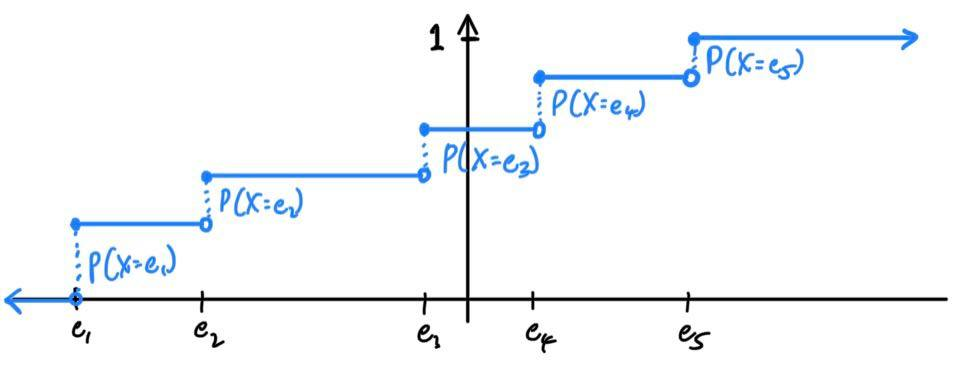
\includegraphics[scale=0.25]{img/Discrete_CDF.jpg}
    \end{center}
    If $E$ was countable, then it would have countably infinite discontinuities. Now we'll give some examples of discrete random variables, and in here we'll completely ignore the sample space $\Omega$, since once we have a random variable $X$, we can just work in $(\mathbb{R}, \mathcal{R}, \mathbb{P}_X)$. Remember that we will write $P(X = x)$ as shorthand for $\mathbb{P}_X (\{x\})$. 

    \begin{definition}[Indicator/Bernoulli Random Variable]
      Given $(\Omega, \mathcal{F}, \mathbb{P})$, let $A \in \mathcal{F}$ be an event. A useful random variable is the \textbf{indicator random variable} $1_A: \Omega \longrightarrow \mathbb{R}$ defined  
      \begin{equation}
        1_A (\omega) = \begin{cases} 1 & \text{ if } \omega \in A \\ 0 & \text{ if } \omega \not\in A \end{cases}
      \end{equation}
      This is a random variable since the preimages of $\emptyset, \{0\}. \{1\}, \{0, 1\}$ are $\emptyset, A^c, A, \Omega$, which are all $\mathcal{F}$-measurable. Since the probability measure of $A$ is $\mathbb{P}(A) = p$, then $\mathbb{P}(A^c) = 1 - \mathbb{P}(A) = 1 - p$, and so we get the PMF 
      \begin{equation}
        p_{1_A} (x) = \begin{cases} 1 - p & \text{ if } x = 0 \\ p & \text{ if } x = 1 \end{cases}
      \end{equation}
      The CDF of this function will look like a step function 
      \begin{equation}
        F_{1_A} (x) = \begin{cases} 0 & \text{ if } x < 0  \\ P(A^c) & \text{ if } 0 \leq x < 1 \\ 1 & \text{ if } 1 \leq x \end{cases}
      \end{equation}
    \end{definition}

    \begin{example}[Uniform Random Variable]
      Given a finite set $E = \{e_i\}_{i=1}^n \subset \mathbb{R}$, we define the PMF as 
      \begin{equation}
        p_X (e_i) = \mathbb{P}(X = e_i) = \frac{1}{n} \; \forall i = 1, 2, \ldots n
      \end{equation}
      which induces the probability measure $\mathbb{P}_X (B) = \sum_{x \in E \cap B} p_X (x)$. 
    \end{example}

    The Bernoulli RV leads to the geometric and binomial random variables. 

    \begin{example}[Geometric Random Variable]
      Given $E = \mathbb{N}$, we can define the PMF associated with random variable $X \sim \mathrm{Geometric}(p)$ as 
      \begin{equation}
        p_X (k) =\mathbb{P}(X = k) = (1 - p)^{k-1} p \text{ for } k \in \mathbb{N}, \; p \in [0, 1]
      \end{equation}
      which induces the probability measure $\mathbb{P}_X (B) = \sum_{x \in E \cap B} p_X (x)$. We can interpret this as the number of times you have to (independently) toss a $p$-coin (probability of heads is $p$) until you get a heads. 
    \end{example}

    \begin{example}[Binomial Random Variable]
      We let $E = \mathbb{N}_0$ and define the PMF associated with random variable $X \sim \mathrm{Binomial}(n, p)$ as 
      \begin{equation}
        p_X (k) = \mathbb{P}(X = k) = \binom{n}{k} p^k (1 - p)^{n - k} \text{ for } k \in E, p \in [0, 1]
      \end{equation}
      We can interpret this as the number of heads occurring in a sequence of $n$ independent tosses of a $p$-coin. 
    \end{example}

    \begin{example}[Poisson Random Variable]
      We let $E = \mathbb{N}_0$ and define the PMF of $X \sim \mathrm{Poisson}(\lambda)$ as 
      \begin{equation}
        p_X (k) = \frac{e^{-\lambda} \lambda^k}{k!} \text{ for } k \in E, \; \lambda > 0
      \end{equation}
    \end{example}

    \begin{definition}[Negative Binomial Distribution]
      The negative binomial distribution, denoted NB$(r, p)$ is defined as
      \begin{equation}
        \mathbb{P}(X = x) \equiv \binom{k+r-1}{k} \, (1-p)^r \, p^k
      \end{equation}
      It can be interpreted as the distribution that models the number of successes in a sequence of iid Bernoulli-$p$ trials before a specified number $r$ failures occurs. 
    \end{definition}

    A slight generalization of a discrete random variable is a simple random variable. Recall that the indicator random variable is a function $1_A: \Omega \rightarrow \mathbb{R}$ defined 
    \begin{equation}
      1_A (\omega) \coloneqq \begin{cases} 1 & \text{ if } \omega \in A \\
      0 & \text{ if else } \end{cases}
    \end{equation}
    As simple random variable generalizes this into multiple sets that form a partition of $\Omega$. It is analogous to a simple function, introduced in measure theory. 

    \begin{definition}[Simple Random Variable]
      Let $\{A_i\}_i$ form a partition of probability space $\Omega$. A \textbf{simple random variable} $X$ is a random variable of the form 
      \begin{equation}
        X (\omega) = \sum_{i} a_i 1_{A_i} (\omega)
      \end{equation}
      that assigns value $a_i$ if the input $\omega \in A_i$. 
    \end{definition}

    Now, let's move on to continuous random variables. 

    \begin{definition}[Absolutely Continuous Measures]
      Let $\mu, \nu$ be measures defined on $(\Omega, \mathcal{F})$. We say that $\nu$ is \textbf{absolutely continuous} w.r.t. $\mu$ if for every $N \in \mathcal{F}$ s.t. $\mu(N) = 0$, we have $\nu(N) = 0$. 
    \end{definition}

    \begin{definition}[Continuous Random Variable]
      A random variable $X$ is \textbf{continuous} if its induced measure $\mathbb{P}_X: (\mathbb{R}, \mathcal{R}) \rightarrow [0, 1]$ is absolutely continuous w.r.t. the Lebesgue measure $\lambda: (\mathbb{R}, \mathcal{R}) \rightarrow \mathbb{R}$, i.e. if for every Borel set $N$ of Lebesgue measure $0$, we have $\mathbb{P}_X (N) = 0$ also. 
    \end{definition}

    A common misconception is that a random variable $X$ is continuous if the induced measure on every singleton set in $\mathcal{B}(R)$ is $0$, i.e. $\mathbb{P}_X (\{x\}) = 0$ for all $x \in \mathbb{R}$. The definition above implies this since the Lebesgue measure of every singleton set is $0$. 

    We introduce a theorem that is useful to know, but we won't prove it. 

    \begin{theorem}[Radon-Nikodym Theorem (Special Case)]
      Let $X$ be a continuous random variable. Then, there exists a nonnegative measurable function $f_X : \mathbb{R} \longrightarrow [0, \infty)$ s.t. for any $B \in \mathcal{R}$, we have 
      \begin{equation}
        \mathbb{P}_X (B) = \int_B f_X \, d\lambda
      \end{equation}
      where the above is the Lebesgue integral. Note that we must define using the Lebesgue integral because Riemann integral is not compatible with any Borel set. $f_X$ is called the \textbf{probability density function}, aka \textbf{PDF}. Furthermore, we can get $f_X$ from $\mathbb{P}_X$ by taking the \textbf{Radon-Nikodym derivative} (which we will not define now)
      \begin{equation}
        f_X = \frac{d \mathbb{P}_X}{d \lambda}
      \end{equation}
      which basically says that if we have a set of very small Lebesgue measure $d \lambda$ tending to $0$, then its probability measure $\mathbb{P}_X$ will also be very small, and the infinitesimal ratio of these two measures on an arbitrarily small set is $f_X$. Also, note that the integral does not change if the value of $f$ changes on sets of Lebesgue measure $0$, and so there is no unique PDF describing $\mathbb{P}_X$. It is unique up to sets of Lebesgue measure $0$, so when we refer to such a PDF $f_X$, we are really talking about an equivalence class of functions. 
    \end{theorem}

    This theorem guarantees the existence of some $f_X$ that completely describes the probability law $P_X$! Take a special case of when $B = (-\infty, x])$, and we can define the CDF as 
    \begin{equation}
      F_X (x) = P_X ((-\infty, x]) = \int_{(-\infty, x]} f_X \, d\lambda
    \end{equation}
    If the set of integration is an interval (and the function is continuous a.e.), then the Lebesgue integral and Riemann integral coincides, and we get the familiar formula 
    \begin{equation}
      F_X (x) = \int_{-\infty}^x f_X (t)\,dt
    \end{equation}
    and we can differentiate it to get back the PDF $f_X$ (or more accurately, some function that agrees with $f_X$ a.e.). We can show that the CDF of a continuous random variable $X$
    \begin{enumerate}
      \item is absolutely continuous, and 
      \item is differentiable almost everywhere, which means that its PDF will be defined almost everywhere (and we can fill in the undefined points however we want). 
    \end{enumerate}
    Note that the PDF $f_X$ itself has no interpretation as a probability (indeed, we can change its value at a countable number of points to anything we want). It is only when we integrate it over some Borel set that gives us a probability. 

    \begin{example}[Uniform Random Variable]
      Let us define the uniform probability measure $P_X$ on $(\mathbb{R}, \mathcal{R})$ with the CDF 
      \begin{equation}
        F_X = \begin{cases} 0 & \text{ if } x < 0 \\
        x & \text{ if } 0 \leq x \leq 1 \\
        1 & \text{ if } 1 < x \end{cases}
      \end{equation}
      It is differentiable almost everywhere except for at the two points $x = 0$ and $x = 1$. Therefore, the PDF $f_X$ is defined for all real numbers except $x = 0$ and $x = 1$. But it doesn't matter: we can assign any value $f_X$ we want on $0$ and $1$ since it won't affect the integral of it. In this example, we just set 
      \begin{equation}
        f_X = \begin{cases} 1 & \text{ if } 0 \leq x \leq 1 \\
        0 & \text{ if else} \end{cases} 
      \end{equation}
    \end{example}

    \begin{example}[Exponential Random Variable]
      The exponential random variable has the following CDF: 
      \begin{equation}
        F_X (x) = \begin{cases} 1 - e^{-\lambda x} & \text{ if } x \geq 0 \\ 0 & \text{ if } x < 0 \end{cases} \text{ for } \lambda > 0
      \end{equation}
      which is differentiable everywhere except at $x = 0$. Differentiating it (and assigning a convenient value at $x = 0$ $f(0) = \lambda$) gives the PDF 
      \begin{equation}
        f_X (x) = \begin{cases} \lambda e^{-\lambda x} & \text{ if } x \geq 0 \\ 0 & \text{ if else} \end{cases}
      \end{equation}
    \end{example}

    \begin{example}[Gaussian Random Variable]
      The PDF is easier to specify for the Gaussian, so we define the Gaussian RV as having PDF 
      \begin{equation}
        f_X (x) = \frac{1}{\sigma \sqrt{2 \pi}} \exp \bigg( -\frac{(x - \mu)^2}{2 \sigma^2} \bigg) \text{ for } \mu \in \mathbb{R}, \sigma > 0
      \end{equation}
      Note that this PDF decreases very quickly as we get further from $\mu$. The CDF cannot be written in closed form, and we call the CDF of the standard Gaussian the \textbf{error function}: 
      \begin{equation}
        \mathrm{Erf}(x) = F_X (x) = \int_{-\infty}^x \frac{1}{\sqrt{2 \pi}} e^{- t^2 / 2} \, dt
      \end{equation}
    \end{example}

    \begin{example}[Cauchy Random Variable (Standardized)]
      The Cauchy random variable gives the PDF 
      \begin{equation}
        f_X (x) = \frac{1}{\pi} \frac{1}{1 + x^2} \text{ for } x \in \mathbb{R}
      \end{equation}
      Integrating this gives the inverse tangent, which after scaling it down by $\pi$ satisfies the conditions of the CDF. Note that the Cauchy distribution falls off much more slowly around the mean (at a rate of $\frac{1}{1 + x^2}$, like a power law) than the Gaussian (which is even \textit{faster} than an exponential, it is at the rate of $e^{-x^2}$). If such a PDF falls off at a slow rate, like a power law, then this is called a \textit{heavy-tailed random variable}. 
    \end{example}

    \begin{example}[Gamma Random Variable]
      The PDF associated with random variable $X \sim \mathrm{Gamma}(n, \lambda)$ is defined 
      \begin{equation}
        f_X(x) = \frac{\lambda^n x^{n-1}}{\Gamma(n)} e^{-\lambda x} \text{ for } x \geq 0
      \end{equation}
      where $\Gamma$ is the gamma function, which is an extension of the factorial function to the domain of complex numbers. 
      \begin{equation}
        \Gamma(x) \coloneqq \int_{0}^\infty z^{x-1} e^{-z}\, dz, \;\;\;\;\; \text{Re}(x) > 0
      \end{equation}
    \end{example}

    \begin{example}[Beta Random Variable]
      The PDF associated with random variable $X \sim \mathrm{Beta}(\alpha, \beta)$, for positive reals $\alpha, \beta$, is defined 
      \begin{equation}
        f_X (x) \equiv \frac{x^{\alpha-1} \,(1-x)^{\beta-1}}{B(\alpha, \beta)}, \text{ where } B(\alpha, \beta) \equiv \frac{\Gamma(\alpha) \Gamma(\beta)}{\Gamma(\alpha + \beta)}
      \end{equation}
      and $\Gamma$ is the Gamma function. 
    \end{example}

    \begin{example}[Uniform RV defined on Cantor Set]
      The cantor set $C \subset [0, 1]$ is defined by removing $(1/3, 2/3)$ from $[0, 1]$ and then removing the middle third from each interval that remains. We define the distribution on this set by defining its CDF: We set 
      \begin{enumerate}
        \item $F(x) = 0$ for $x \leq 0$ and $F(x) = 1$ for $x \geq 1$. 
        \item $F(x) = 1/2$ for $x \in [1/3, 2/3]$, 
        \item $F(x) = 1/4$ for $x \in [1/9, 2/9]$ and $F(x) = 3/4$ for $x \in [7/9, 8/9]$, ... 
      \end{enumerate}
      and extend $F$ to all of $[0 ,1]$ using monotonicity. 
    \end{example} 

    \begin{example}[Dense Discontinuities]
      Let $q_1, q_2, \ldots$ be an enumeration of the rationals. Let $\alpha_i > 0$ have $\sum_{i=1}^\infty \alpha_i = 1$, and let 
      \begin{equation}
        F(x) = \sum_{i=1}^\infty \alpha_i 1_{[q_i, \infty)} (x)
      \end{equation}
      where $1_{[q_i, \infty)} (x) = 1$ if $x \in [q_i, \infty)$ and $0$ if otherwise. 
    \end{example}

    To summarize, once we have a random variable $X: \Omega \rightarrow \mathbb{R}$, we can throw away the sample space and work in $(\mathbb{R}, \mathcal{R}, \mathbb{P}_X)$ with the induced measure $\mathbb{P}_X$, which is known as the \textbf{probability distribution} of $X$.  
    \begin{enumerate}
      \item If $X$ is discrete, then let there be some at most countable set $E = \{e_i\}$ where $P(E) = 1$. it turns out that $\mathbb{P}_X$ can be completely defined by a probability mass function $p_X : \mathbb{R} \rightarrow \mathbb{R}$ defined 
      \begin{equation}
        p_X (x) = \mathbb{P}_X (\{x\}).
      \end{equation}
      Given that we have this PMF , we can define $\mathbb{P}_X$ as such: Given any Borel $B \in \mathcal{R}$, 
      \begin{equation}
        \mathbb{P}_X (B) = \sum_{x \in E \cap B} p_X (x)
      \end{equation}
      \item If $X$ is continuous, then the Radon-Nikodym Theorem asserts the existence of a nonnegative probability density function $f_X$ that completely describes the probability law $\mathbb{P}_X$. Given that we have this PDF, we can then define $\mathbb{P}_X$ as such: Given any Borel $B \in \mathcal{R}$, 
      \begin{equation}
        \mathbb{P}_X (B) = \int_B f_X \, d\lambda
      \end{equation}
    \end{enumerate}

  \subsubsection{Space of Measurable Functions}

    Now it turns out that the space of $\mathcal{F}$-measurable functions $X: \Omega \rightarrow \mathbb{R}$ forms a function space, which means that the set of all random variables on $\Omega$ forms a vector space. We formally show it here. 

    \begin{lemma}
      The set of all $\mathcal{F}$-measurable functions $X: (\Omega, \mathcal{F}) \rightarrow \mathbb{R}$ forms a vector space, denoted $L_\mathcal{F} (\Omega; \mathbb{R})$, or $L_\mathcal{F} (\Omega)$ for short. 
    \end{lemma}
    \begin{proof}

    \end{proof}

    Naturally, we can put the $L^p$-norm on this space, defined 
    \begin{equation}
      ||X||_p \coloneqq \bigg( \int_\Omega |X|^p \, d\mathbb{P} \bigg)^{1/p}
    \end{equation}
    Moreover, if $p = 2$, then we can put an inner product defined 
    \begin{equation}
      \langle X, Y \rangle = \bigg( \int_\Omega X Y \,d \mathbb{P} \bigg)^{1/2}
    \end{equation}

    \begin{definition}
      The Banach space of $\mathcal{F}$-measurable functions is denoted $L_\mathcal{F}^p (\Omega)$, and the Hilbert space is denoted $L_\mathcal{F}^2 (\Omega)$. 
    \end{definition}

    This means that if we have some probability space $(\Omega, \mathcal{F}, \mathbb{P})$ and  sub-$\sigma$-algebra $\mathcal{G} \subset \mathcal{F}$, then any $\mathcal{G}$-measurable function is also $\mathcal{F}$-measurable, since if the preimage of every $B \in \mathcal{R}$ is in $\mathcal{G}$, then it $B \in \mathcal{F}$. This immediately results in the following. 

    \begin{theorem}
      If $\mathcal{G}$ is a sub-$\sigma$-algebra of $\mathcal{F}$, then $L_\mathcal{G} (\Omega)$ is a subspace of $L_\mathcal{F} (\Omega)$. 
    \end{theorem}

    This means that as we get coarser and coarser random variables, the space in which these random variables live in get smaller and smaller, until we get to the constant random variables, which form a $1$-dimensional line in $L_\mathcal{F} (\Omega)$. The origin is simply the constant $0$ random variable. 

\subsection{Independence}

  \begin{definition}[Independence of $2$ Events]
    Given probability space $(\Omega, \mathcal{F}, \mathbb{\mathbb{P}})$, events $A, B \in \mathcal{F}$ are said to be \textbf{independent under $\mathbf{\mathbb{P}}$} if 
    \begin{equation}
      \mathbb{P}(A \cap B) = \mathbb{P}(A) \, \mathbb{P}(B)
    \end{equation}
    This leads to the immediate property that if $\mathbb{P}(B) > 0$, with $A, B$ independent, then 
    \begin{equation}
      \mathbb{P}(A \mid B) = \mathbb{P}(A)
    \end{equation}
  \end{definition}

  Note that $A$ and $B$ may be independent under one measure, but not under another measure. The property that $\mathbb{P}(A \mid B) = \mathbb{P}(A)$ is \textit{not} the definition of independence, since it has the more restricting property that $\mathbb{P}(B) > 0$, so only refer to the definition that $\mathbb{P}(A \cap B) = \mathbb{P}(A) \, \mathbb{P}(B)$. This is the true definition of independent events that we should rely on, not the one that says that $A$ and $B$ are independent if "one does not affect the other." This old definition is misleading and false. For example, take the probability space $[0, 1]$, with Borel $\sigma$-algebra, and Lebesgue measure $\mathbb{P} = \lambda$, and let $A = \mathbb{Q}$ and $B = \mathbb{R} \setminus \mathbb{Q}$. Then, contradictory to our old definition, $A$ and $B$ are independent since $\mathbb{P}(A \cap B) = \mathbb{P}(A) \, \mathbb{P}(B) = 0$! By the definition, an event $A$ is independent of itself if $\mathbb{P}(A) = 0$ or $1$ (e.g. $A$ is rationals, irrationals, cantor set, $\emptyset$, $\Omega$, etc.). 

  \begin{definition}[Independence of $n$ Events]
    Given probability space $(\Omega, \mathcal{F}, \mathbb{P})$, 
    \begin{enumerate}
      \item Let us have a finite collection of events $A_1, A_2, \ldots, A_n \in \mathcal{F}$. They are \textbf{independent} if for all nonempty $I_0 \subset \{1, 2, \ldots n\}$, 
      \begin{equation}
        \mathbb{P} \bigg( \bigcap_{i \in I_0} A_i \bigg) = \prod_{i \in I_0} \mathbb{P}(A_i)
      \end{equation}
      Note that it is not enough to just prove that 
      \begin{equation}
        \mathbb{P}(A_1 \cap \ldots \cap A_n) = \prod_{i=1}^n \mathbb{P}(A_i)
      \end{equation}
      We must verify this for all $2^n$ possible choices (to be precise, we don't need to prove for $I_0 = \emptyset$ and $I_0 = \{A_i\}$), so for $2^n - n - 1$ choices. 
      
      \item Let $\{A_i\}_{i \in I}$ be a collection of events indexed by a possibly uncountable $I$. They are independent if for all nonempty and finite $I_0 \subset I$, we have 
      \begin{equation}
        \mathbb{P} \bigg( \bigcap_{i \in I_0} A_i \bigg) = \prod_{i \in I_0} \mathbb{P}(A_i)
      \end{equation}
    \end{enumerate}
  \end{definition}

  Now when we are trying to compare two $\sigma$-algebras, the measure defined for one may not even be defined on the other. To ensure that a measure is defined on both, it makes sense to take its $\sigma$-algebra and construct two sub-$\sigma$-algebras, which $\mu$ is guaranteed to be defined on. 

  \begin{definition}[Independence of $\sigma$-Algebras]
    Let us have probability space $(\Omega, \mathcal{F}, \mathbb{P})$. 
    \begin{enumerate}
      \item Let $\mathcal{F}_1, \mathcal{F}_2$ be two sub-$\sigma$-algebras of $\mathcal{F}$. $\mathcal{F}_1$ and $\mathcal{F}_2$ are independent if for any $A_1 \in \mathcal{F}_1, A_2 \in \mathcal{F}_2$, $A_1$ and $A_2$ are independent. 
      \item Let $\{ \mathcal{F}_i\}_{i \in I}$ be an arbitrary collection of sub-$\sigma$-algebras of $\mathcal{F}$, indexed by possibly uncountable $I$. Then, they are independent if for any choices of $A_i \in \mathcal{F}_i$ for $i \in I$, $\{A_i\}_{i \in I}$ are independent events. 
    \end{enumerate}
  \end{definition}

  \begin{definition}[Independent Random Variables]
    Two random variables $X, Y$ are \textbf{independent} if $\sigma(X)$ and $\sigma(Y)$ are independent $\sigma$-algebras. That is, for any Borel sets $B_1, B_2 \in \mathcal{R}$, the events $X^{-1}(B_1)$ and $Y^{-1}(B_2)$ are independent: 
    \begin{equation}
      \mathbb{P}\big[ X^{-1}(B_1) \cap Y^{-1}(B_2) \big] = \mathbb{P}(X^{-1}(B_1)) \, \mathbb{P}(Y^{-1}(B_2))
    \end{equation}
    or by abusing notation, 
    \begin{equation}
      \mathbb{P}(X \in B_1, Y \in B_2) = \mathbb{P}(X \in B_1) \, \mathbb{P}(Y \in B_2)
    \end{equation}
  \end{definition}

  If $X, Y$ are independent, then we can say something about the CDFs 
  \begin{equation}
    F_{X, Y} (x, y) = F_X (x) \, F_Y (y)
  \end{equation}
  In fact, we can say something stronger. 

  \begin{theorem}
    $X$ and $Y$ are independent RVs if and only if 
    \begin{equation}
      F_{X, Y} (x, y) = F_X (x) \, F_Y (y)
    \end{equation}
  \end{theorem}

  Moving onto multiple variables, we can define that $X_1, X_2, \ldots, X_n$ are independent RVs if $\sigma(X_1), \ldots, \sigma(X_n)$ are independent $\sigma$-algebras. 

\subsection{Functions of Random Variables}

  In many applications, it happens that we are interested not in the value of the random variable $X$, but a function of it. That is, given a probability space $(\Omega, \mathcal{F}, \mathbb{P})$, let us have a random variable $X: \Omega \rightarrow \mathbb{R}$. We can then define another function $f: \mathbb{R} \rightarrow \mathbb{R}$ and consider the potential random variable $f \circ X : \Omega \rightarrow \mathbb{R}$. We say potential because we don't know yet whether $f \circ X$ is measurable (i.e. the preimage of every Borel set in $\mathbb{R}$ is in $\mathcal{F}$). This condition suffices if $f$ itself is a measurable function, i.e. for every Borel set $B \in \mathcal{R}$, its preimage $f^{-1} (B)$ is Borel in $\mathbb{R}$, and by measurablility of $X$, its preimage under $X$ is $\mathcal{F}$-measurable, making $f \circ X$ a viable random variable. With this new random variable $f \circ X$, we would now like to answer the question: What is the probability law $\mathbb{P}_{f \circ X}$ of $\mathbb{R}$? 

  This also works for joint random variables, which we will learn later. Given a joint random variable $(X_1, X_2, \ldots X_n): \Omega \rightarrow \mathbb{R}^n$, we can define a measurable function $f: \mathbb{R}^n \longrightarrow \mathbb{R}$ and define the scalar random variable $f \circ (X_1, \ldots X_n)$ on $\Omega$. But again, we want to find what the CDF of this composition. 

  \subsubsection{Maximum/Minimum of Random Variables}

    Let $X_1, X_2, \ldots, X_n$ be random variables of $(\Omega, \mathcal{F}, \mathbb{P})$ with joint CDF $F_{X_1 \ldots X_n} (x_1, \ldots, x_n)$. Let $Y_n = \min (X_1, \ldots, X_n)$ and $Z_n = \max(X_1, \ldots, X_n)$. Note that $Y_n$ and $Z_n$ are also functions of $\Omega$ to $\mathbb{R}$. To prove that they are random variables, we just have to prove that $\min$ and $\max$ are measurable functions from $\mathbb{R}^n$ to $\mathbb{R}$, which we can do by proving that the preimage of all semi-infinite interval $(-\infty, x]$ are Borel in $\mathbb{R}^n$. 
    \begin{enumerate}
      \item The preimage of $(-\infty, x]$ under $\max$ is just the set of all $n$-vectors whose max is less than $x$, which is just the semi-infinite cuboid $(-\infty, x]^n \subset \mathbb{R}^n$, which is Borel in $\mathbb{R}^n$. 
      \item The preimage of $(-\infty, x]$ under $\min$ is the set of all $n$-vectors whose min is less than $x$, i.e. at least one element must be less than $x$. But this is just the complement of all vectors that have elements all greater than $x$, which is $\mathbb{R}^n \setminus (x, +\infty)^n \subset \mathbb{R}^n$, which is Borel in $\mathbb{R}^n$. 
    \end{enumerate}
    Now we must determine the CDF of $Y_n$ and $Z_n$. 
    \begin{enumerate}
      \item We have 
      \begin{align*}
        F_{Z_n} (z) & = \mathbb{P}(\{ \omega \mid Z_n (\omega) \leq z \}) \\
        & = \mathbb{P}(\{ \omega \mid X_1 (\omega) \leq z, \ldots, X_n (\omega) \leq z\}) \\
        & = F_{X_1 \ldots X_n} (z, \ldots, z)
      \end{align*}
      where the last equality is describes simply the joint CDF of the joint distribution $(X_1, \ldots, X_n)$. If we assume independence of $X_i$'s, it simplifies out to 
      \begin{equation}
        \prod_{i} F_{X_i} (z)
      \end{equation}
      and if iid, then we have $[F_{X} (z) ]^n$, where $X$ is the common distribution. 
      \item For $Y_n$, we work with complements again and have 
      \begin{align*}
        F_{Y_n} (y) & = \mathbb{P}(\{ \omega \mid Y_n (\omega) \leq y \}) \\ 
        & = 1 - \mathbb{P}(\{ \omega \mid Y_n (\omega) > y \}) \\
        & = 1 - \mathbb{P}(\{ \omega \mid X_1 (\omega) > y, \ldots X_n (\omega) > y \}) \\
      \end{align*}
      where $\mathbb{P}(\{ \omega \mid X_1 (\omega) > y, \ldots X_n > y \})$ can be calculated from the joint distribution. If we assume independence of $X_i$, it simplifies out to 
      \begin{equation}
        1 - \prod_{i} \mathbb{P}(\{\omega \mid X_i(\omega) > y \}) = 1 - \prod_{i} \big( 1 - F_{X_i} (y) \big)
      \end{equation}
      and if iid, then we have $1 - [1 - F_{X} (y)]^n$. 
    \end{enumerate}

    \begin{example}[Uniforms]
      Let $X_1, X_2$ be iid distributed as $\mathrm{Uniform}[0, 1]$, and let $Z = \max(X_1, X_2)$ with $Y = \min(X_1, X_2)$, i.e. $Z$ is the greater of the two and $Y$ is the lesser. We would expect the PDF of $Z$ to have more mass towards $1$ and the PDF of $Y$ to have more mass towards $0$. Our common CDF is 
      \begin{equation}
        F_{X} (x) = \begin{cases} 0 & \text{ if } x < 0 \\
        x & \text{ if } 0 \leq x \leq 1 \\
        1 & \text{ if } 1 < x \end{cases}
      \end{equation}
      Let's calculate the CDF of $Z$. 
      \begin{align*}
        F_{Z} (z) & = \mathbb{P}(\{\omega \mid Z(\omega) \leq z\}) \\
        & = \mathbb{P}(\{ \omega \mid X_1 (\omega) \leq z, X_2 (\omega) \leq z\}) \\
        & = F_{X_1, X_2} (z, z) \\
        & = [F_{X} (z)]^2 = \begin{cases} 0 & \text{ if } x < 0 \\
        x^2 & \text{ if } x \in [0, 1] \\
        1 & \text{ if } 1 < x \end{cases}
      \end{align*}
      This CDF is differentiable everywhere except the two points $0$ and $1$, so we can get the PDF to be $f_Z (z) = 2 z$ for $z \in (0, 1)$ and $0$ otherwise. For the values of $f_Z$ at $0$ and $1$, we can fill it in with anything we want (since the measure of these sets are $0$), so we will just defined $f_Z (0) = 0$ and $f_Z(1) = 2$, getting 
      \begin{equation}
        f_Z (z) = \begin{cases} 2 z & \text{ if } z \in [0, 1] \\
        0 & \text{ if else} \end{cases}
      \end{equation}
      Let's calculate the CDF of $Y$. 
      \begin{align*}
        F_{Y} (y) & = \mathbb{P}(\{ \omega \mid Y(\omega) \leq y\}) \\
        & = 1 - \mathbb{P}(\{ \omega \mid Y(\omega) > y\}) \\
        & = 1 - \mathbb{P}(\{\omega \mid X_1 (\omega) > y, X_2 (\omega) > y \}) \\
        & = 1 - \mathbb{P}(\{\omega \mid X_1 (\omega) > y\}) \, \mathbb{P}(\{ X_2 (\omega) > y \}) \\ 
        & = 1 - [1 - F_X (y)]^2 = \begin{cases} 0 & \text{ if } y < 0 \\
        1 - (1 - y)^2 & \text{ if } y \in [0, 1] \\
        1 & \text{ if } y > 1 \end{cases} 
      \end{align*}
      and differentiating it (with setting any values of the PDF at the nondifferentiable points $0$ and $1$) gives 
      \begin{equation}
        f_Y (y) = \begin{cases} 2 - 2y & \text{ if } y \in [0, 1] \\
        0 & \text{ if else} \end{cases}
      \end{equation}
    \end{example}

    \begin{example}[Exponentials]
      Let $X_1, X_2, \ldots, X_n$ be independent exponential random variables with parameters $\lambda_1, \ldots, \lambda_n$, respectively (not identical!). Then, for each $X_i$, its CDF is 
      \begin{equation}
        F_{X_i} (x) = 1 - e^{-\lambda_i x} \text{ for } x \geq 0
      \end{equation}
      and let $Y = \min(X_1, \ldots, X_n)$. Then, we have 
      \begin{align*}
        F_Y (y) & = 1 - \prod_{i=1}^n [ 1 - F_{X_i} (y)] \\
        & = 1 - \prod_{i=1}^n e^{-\lambda_i x} \\
        & = 1 - e^{- ( \sum_{i=1}^n \lambda_i ) x}
      \end{align*}
      which is the CDF of an exponential distribution. So, 
      \begin{equation}
        Y \sim \mathrm{Exponential}(\lambda_1 + \ldots + \lambda_n)
      \end{equation}
      This is nice, since the minimum of a bunch of exponentials is an exponential. However, this is not the case for the maximum. 
    \end{example}

    This has nice practical applications. For example, recall the memoryless property of the exponential, which nicely models radioactive decay. If we have $n$ elements each decaying at some $\mathrm{Exponential}(\lambda_i)$ rate, then we can model the time at which the first alpha particle will emit amongst all $n$ elements will also be an exponential. These processes where the inter-emission times are exponentials are called Poisson process, which we will discuss later. 

    \begin{definition}[Order Statistic]
      Let $X_1, X_2, ..., X_n$ be a finite collection of independent, identically distributed random variables. Suppose that they are continuously distributed with density $f$ and CDF $F$. Define the random variable $X_{(k)}$ to be the $k$th ranked value, called the \textbf{$k$th order statistic}. This means that 
      \begin{equation}
        X_{(1)} = \min\{X_1, X_2, ..., X_n\}, \;\; X_{(n)} = \max\{X_1, X_2, ..., X_n\}
      \end{equation}
      and in general, for any $k \in \{1, 2, ..., n\}$, 
      \begin{equation}
        X_{(k)} = X_j \text{ if } \sum_{l=1}^n \mathbb{I}_{X_l < X_j} = k - 1
      \end{equation}
      which means that exactly $k-1$ of the values of $X_l$ are less than $X_j$. Since $F$ is continuous, 
      \begin{equation}
        X_{(1)} < X_{(2)} < ... < X_{(n)}
      \end{equation}
      holds with probability $1$. This leads us to define the random variable $X_{(k)}$ representing the $k$th order statistic.
      \begin{equation}
        f_{(k)} (y) = \begin{cases} 
        n \, \binom{n-1}{k-1} y^{k-1} (1-y)^{n-k} & y \in (0, 1) \\
        0 & y \not\in (0,1)
        \end{cases}
      \end{equation}
      That is, $X_{(k)}$ has the Beta$(k, n-k_1)$ distribution. 
    \end{definition}

  \subsubsection{Convolutions and Sums of Random Variables}

    Now given two random variables $X, Y: \Omega \rightarrow \mathbb{R}$ that each push their own probability laws $\mathbb{P}_X, \mathbb{P}_Y$ onto $\mathbb{R}$, their sum $Z = X + Y$ is also a random variable that pushes its own probability law $\mathbb{P}_Z$. We must actually prove that $Z$ is a random variable, which we can do by proving that the preimage of every $(-\infty, x]$ is $\mathcal{F}$-measurable. Equivalently (by complementation), we must prove that the preimage of every $(x, +\infty)$ (that is, all sets of form $\{ \omega \mid Z(\omega) > z\}$) is $\mathcal{F}$-measurable. Now we can write $z$ as the sum of two numbers $z = q + (z - q)$, where $q \in \mathbb{R}$, and say that 
    \begin{equation}
      \{ \omega \mid Z(\omega) > z\} = \bigcup_{q \in \mathbb{R}} \{ \omega \mid X (\omega) > q , \; Y(\omega) > z - q\}
    \end{equation}
    But using the fact that $\mathbb{Q}$ is dense in $\mathbb{R}$, we can turn this from an uncountable union to a countable union and say 
    \begin{align}
      \{ \omega \mid Z(\omega) > z\} & = \bigcup_{q \in \mathbb{Q}} \{ \omega \mid X (\omega) > q , \; Y(\omega) > z - q\} \\
      & = \bigcup_{q \in \mathbb{Q}} \big( \{\omega \mid X(\omega) > q\} \cap \{ \omega \mid Y(\omega) > z - q\} \big) 
    \end{align}
    and since I have a countable union of (an intersection of) these $\mathcal{F}$-measurable sets, $\{ \omega \mid Z(\omega) > z\}$ is $\mathcal{F}$-measurable, and we are done. This equation above even gives us a hint of how to compute the CDF of $Z$. 

    \begin{theorem}
      Given random variables $X_1, X_2, \ldots, X_n$ of probability space $(\Omega, \mathcal{F}, \mathbb{P})$, 
      \begin{enumerate}
        \item $X_1 + \ldots + X_n$ is a random variable.
        \item $X_1 \cdot \ldots \cdot X_n$ is a random variable. 
      \end{enumerate}
    \end{theorem}

    For simplicity, we will only consider jointly discrete or jointly continuous random variables. The probability law $\mathbb{P}_Z$ can be confusing to define, since given some Borel set $B \in \mathcal{R}$, we must now look at the preimage under the \textit{sum} $X + Y$. A simpler way to approach this is to consider the joint distribution $X, Y$ and look at its distribution, which we call the \textbf{convolution} of $X$ and $Y$. This is especially simple to consider for discrete random variables. 

    \begin{definition}[Sums of Discrete Random Variables]
      Take two discrete random variables $X, Y$ with their joint PMF $p_{X, Y} (x, y)$ and their sum $Z = X + Y$. We can see that the PMF of $Z$ is 
      \begin{equation}
        p_Z (z) = \sum_{(x, y) \,:\, x + y = z} p_{X, Y} (x, y) = \sum_{x \in \mathcal{X}} p_{X, Y} (x, z - x)
      \end{equation}
      which by abuse of notation, we denote
      \begin{equation}
        \mathbb{P}(Z = z) = \sum_{x \in \mathcal{X}} \mathbb{P}(X = x, Y = z - x)
      \end{equation}
      The CDF is very simple, since we just have to sum over all $(x, y)$ such that their sum is less than $z$: 
      \begin{equation}
        F_Z (z) = \sum_{(x, y) \,:\, x + y \leq z} p_{X, Y} (x, y)
      \end{equation}
      which by abuse of notation, we write 
      \begin{equation}
        \mathbb{P}(Z \leq z) = \sum_{(x, y) \,:\, x + y \leq z} \mathbb{P}(X = x, Y = y)
      \end{equation}
      If $X$ and $Y$ are independent, then their joint distribution is the product of their singular distributions, and so we have 
      \begin{equation}
        p_Z (z) = \sum_x p_X (x) \, p_Y (z - x) \coloneqq p_X \ast p_Y
      \end{equation}
      where $p_Z = p_X \ast p_Y$ is called the convolution of $p_X$ and $p_Y$. By abuse of notation, 
      \begin{equation}
        \mathbb{P}(Z = z) = \sum_{x \in \mathcal{X}} \mathbb{P}(X = x) \, \mathbb{P}(Y = z - x)
      \end{equation}
    \end{definition}

    \begin{example}[Sums of Poisson RVs]
      Let $X_1$ and $X_2$ be independent Poisson random variables with parameters $\lambda_1, \lambda_2 > 0$, and let $Z = X_1 + X_2$. The PMF of each $X_i$ is 
      \begin{equation}
        p_{X_i} (k) = \frac{e^{-\lambda_i} \lambda_i^k}{k!} \text{ for } k \in \mathbb{Z}
      \end{equation}
      and taking the convolution gives the PMF of $Z$: 
      \begin{align*}
        p_Z (z) & = (p_{X_1} \ast p_{X_2}) (z) \\
        & = \sum_{k=-\infty}^{+\infty} \frac{e^{-\lambda_1} \lambda_1^k}{k!} \cdot \frac{e^{-\lambda_2} \lambda_2^{z - k}}{(z - k)!} \\
        & = \sum_{k=0}^{z} \frac{e^{-\lambda_1} \lambda_1^k}{k!} \cdot \frac{e^{-\lambda_2} \lambda_2^{z - k}}{(z - k)!} \\ 
        & = \frac{e^{-(\lambda_1 + \lambda_2)}}{z!} \sum_{k=0}^z \binom{z}{k} \lambda_1^k \lambda_2^{z - k} \\
        & = \frac{e^{-(\lambda_1 + \lambda_2)} (\lambda_1 + \lambda_2)^z}{z!} 
      \end{align*}
      for $z \in \mathbb{N}_0$, which is the PMF of another Poisson. So, $Z \sim \mathrm{Poisson}(\lambda_1 + \lambda_2)$. 
    \end{example}

    This has a nice visualization, since the joint distribution of $X$ and $Y$ over $\mathbb{R}^2$ is being "summed up/integrated" over the diagonals of $\mathbb{R}^2$, i.e. the lines where $x + y = z$ for some $z$, sort of like marginalizing over these diagonals. This creates a new "diagonally marginal distribution" $Z$. 

    \begin{definition}[Sums of Continuous Random Variables]
      Take two continuous random variables $X, Y$ with their joint PDF $f_{X, Y} (x, y)$ and their sum $Z = X + Y$. To calculate the CDF, we must basically integrate the joint PDF over the borel set $\{(x, y) \in \mathbb{R}^2 \mid x + y \leq z\}$. 
      \begin{align*}
        \mathbb{P}(Z \leq z) = F_Z (z) & = \int_{(x, y) \,:\, x + y \leq z} f_{X, Y} (x, y) \,dy\,dx \\
        & = \int_{-\infty}^{+\infty} \int_{-\infty}^{z - x} f(x, y) \,dy \,dx
      \end{align*}
      We can see that the PDF of $Z$ is 
      \begin{equation}
        f_{Z} (z) = \int_{\mathbb{R}} f_{X, Y} (x, z - x) \, dx
      \end{equation}
      If $X$ and $Y$ are independent, then 
      \begin{equation}
        f_{Z} (z) = \int_{\mathbb{R}} f_{X} (x) \, f_Y (z - x) \,dx \coloneqq f_X \ast f_Y
      \end{equation}
      where $f_Z = f_X \ast f_Y$ is the convolution of $f_X$ and $f_Y$. 
    \end{definition}

    \begin{definition}[Convolution]
      Given two functions $f, g: \mathbb{R} \longrightarrow \mathbb{R}$, the \textbf{convolution} of $f$ and $g$ is a new function $f \ast g$ defined  
      \begin{equation}
        (f \ast g) (t) \coloneqq \int_\mathbb{R} f(t)\, g(t - \tau) \, d \tau
      \end{equation}
    \end{definition}

    Usually, when we take convolutions, it is not pretty and even for nice distributions like two Gaussians, convolving them is quite complicated. What we can do is transform them (using Laplace, Fourier, etc.) to make calculations easier and more elegant, which we will talk about later.  

    \begin{example}
      Let $X_1$ and $X_2$ be independent exponential with parameters $\lambda_1, \lambda_2$, with individual PDFs $f_{X_i} (x) = \lambda_i e^{-\lambda_i x}$ for $x \geq 0$. Let $Z = X_1 + X_2$. Then, 
      \begin{align*}
        f_Z (z) = (f_{X_1} \ast f_{X_2})(z) & = \int_{-\infty}^\infty \lambda_1 e^{-\lambda_1 x} \, \lambda_2 e^{-\lambda_2 (z -x)} \, dx \\
        & = \int_{0}^z \lambda_1 e^{-\lambda_1 x} \, \lambda_2 e^{-\lambda_2 (z -x)} \, dx \\ 
        & = \lambda_1 \lambda_2 e^{-\lambda_2 z} \int_0^z e^{(\lambda_2 - \lambda_1) x}\,dx \\
        & = \begin{cases} \frac{\lambda_1 \lambda_2}{\lambda_2 - \lambda_1} \big( e^{-\lambda_1 z} - e^{-\lambda-2 z} \big) & \text{ if } \lambda_1 \neq \lambda_2 \\
        \lambda^2 z e^{-\lambda z} & \text{ if } \lambda_1 = \lambda_2 = \lambda \end{cases} 
      \end{align*}
      The distribution for when $\mu_1 = \mu_2$ is called the Erlang distribution, which has many applications, but the other case is an ugly form and not studied very well. 
    \end{example}

    \begin{theorem}[Sums of Discrete Variables]
      Assume that $X$ and $Y$ are independent. 
      \begin{enumerate}
        \item $X \sim$ Binomial$(n, p)$, $Y \sim$ Binomial$(m, p)$ $\implies X + Y \sim$ Binomial$(n + m, p)$. 
        \item $X \sim$ Poisson$(\lambda)$, $Y \sim$ Poisson$(\gamma)$ $\implies X + Y \sim$ Poisson$(\lambda + \gamma)$. 
        \item If $X_1, ..., X_n$ are Geometric$(p)$, then $X_1 + ... + X_n$ is NB$(n, p)$. 
      \end{enumerate}
    \end{theorem}

    \begin{theorem}[Sums of Densities]
      Assume that $X$ and $Y$ are independent. 
      \begin{enumerate}
        \item $X \sim$ Normal$(\mu_1, \sigma_1^2)$, $Y \sim$ Normal$(\mu_2, \sigma_2^2)$ $\implies X + Y \sim$ Normal $(\mu_1 + \mu_2, \sigma_1^2 + \sigma_2^2)$. 
        \item If $X_1, X_2, ..., X_n$ are Exponential$(\lambda)$, then $X_1 + ... + X_n \sim$ Gamma$(n, \lambda)$.
        \item $X \sim$ Gamma$(n, \lambda)$, $Y \sim$ Gamma$(m, \lambda)$ $\implies X + Y \sim$ Gamma$(n + m, \lambda)$. 
        \item $X \sim$ Gamma $(n, \lambda)$, $Y \sim$ Exponential $(\lambda)$ $\implies X + Y \sim$ Gamma$(n+1, \lambda)$. 
      \end{enumerate}
    \end{theorem}

  \subsubsection{Sum of Random Number of Random Variables}

    Now we consider a random variable where the number of terms we are summing is a random variable. Let $\{X_i\}_i$ be a countable sequence of independent random variables with CDF $F_{X_i}$. Let $N$ be a positive integer-valued random variable with PMF $p_N(n) = \mathbb{P}(N = n)$. Assume that $N$ is independent of $X_i$'s. Now, consider the function 
    \begin{equation}
      S_N \coloneqq \sum_{i=1}^N X_i
    \end{equation}
    To interpret this, consider the sample space $\Omega$. We have all $X_i$'s and $N$ defined on the same $\Omega$. Once $\omega \in \Omega$ realizes, the $\{X_i\}$'s will realize as a sequence of numbers, and $N$ will realize as a positive integer. We simply sum them up according to the rule $S_N$, and by this definition, $S_N$ is a real-valued function on $\Omega$. We first have to prove that $S_N$ is a random variable (since we only know that a \textit{fixed} sum of random variables is a random variable), and then we must find the CDF of $S_N$ $\mathbb{P}(S_N \leq x)$. 

    First, note that the realization of $N$ partitions the sample space as 
    \begin{equation}
      \Omega = \bigsqcup_{n = 1}^\infty \{\omega \mid N(\omega) = n\}
    \end{equation}
    Once I have this partition, I can invoke the partition rule and write 
    \begin{align*}
      \mathbb{P}(S_N \leq x) & = \sum_{k=1}^\infty \mathbb{P}(S_N \leq x \mid N = k) \, \mathbb{P}(N = k) \\
      & = \sum_{k=1}^\infty \mathbb{P}(S_k \leq x \mid N = k) \, \mathbb{P}(N = k) & (\text{conditioned on } N = k) \\
      & = \sum_{k=1}^\infty \mathbb{P}(S_k \leq x) \, \mathbb{P}(N = k) & (N \text{ is indep. of } X_i \text{s})
    \end{align*}
    where $\mathbb{P}(N = k)$ is known since we know the PMF of $N$, and the CDFs $\mathbb{P}(S_k \leq x)$ can be computed by computing the deterministic sums and computing their CDF. 

    \begin{example}
      Let $X_i$'s be iid $\mathrm{Exponential}(\lambda)$, and $N \sim \mathrm{Geometric}(p)$. We know that the deterministic sum of iid exponentials gives an Erlang. So, $S_N = \sum_{i=1}^N X_i$, and its CDF is 
      \begin{equation}
        \mathbb{P}(S_N \leq x) = \sum_{k=1}^\infty \mathbb{P}(S_k \leq x) \, \mathbb{P}(N = k)
      \end{equation}
      where $\mathbb{P}(N = k) = (1 - p)^{k - 1} p$. The PDF of the Erlang is 
      \begin{equation}
        p_{S_k} (x) = \frac{\lambda^n x^{n-1}}{(n - 1)!} e^{-\lambda x}
      \end{equation}
      and doing the brute force calculations gives a clean $S_N \sim \mathrm{Exponential}(\lambda p)$. 
    \end{example}

  \subsubsection{General Transformations of Random Variables}

    Now we will look at more general transformations that are not just minimum, maximum, deterministic sums, or random sums. Let us have a probability space $(\Omega, \mathcal{F}, \mathbb{P})$, a random variable $X: \Omega \rightarrow \mathbb{R}$, and a measurable function $f: \mathbb{R} \rightarrow \mathbb{R}$. Now given that we know the CDF (and therefore distribution) of $X$, we want to find the CDF of random variable $Y = f(X) = f \circ X$ (which we have established as a random variable already due to measurability of $f$): $F_Y (y) = \mathbb{P}(Y \leq y)$, which is just $\mathbb{P}_Y ((-\infty, y])$ (where $\mathbb{P}_Y$ is the probability law on $Y$). But rather than trying to take the preimage of the entire composite random variable $Y$ and calculating $\mathbb{P}\big( Y^{-1}((-\infty, y]) \big)$ under the probability on $\mathcal{F}$, let's just take the preimage one step at a time. Note that $f^{-1} \big( (-\infty, y] \big) = \{x \in \mathbb{R} \mid f(x) \leq y\}$. We can then write the CDF of $Y$ in terms of the probability law of $X$: 
    \begin{align*}
      F_Y (y) & = \mathbb{P}_X \big( f^{-1} ((-\infty, y]) \big) \\
      & = \mathbb{P}_X \big( \{x \in \mathbb{R} \mid f(x) \leq y\} \big) \\
      & = \mathbb{P} \big( X^{-1} \circ f^{-1} ((-\infty, y]) \big) 
    \end{align*}
    Depending on how complicated $f$ is, this may be easy or not, but conceptually, this is no problem. But theoretically, this is as far as we can go. Let's move onto some examples. We start with a practical way to generate a Gaussian distribution, which is how most modern software computes. 

    \begin{example}[Box-Muller Transform]
      Given that you have a uniform random number generator in $[0, 1]$, you can generate a normal $N(0, 1)$ by transforming it using the inverse CDF of the normal. This is usually computationally heavy since the inverse CDF of the Gaussian requires expensive operations. An easier way is to use the \textbf{Box-Muller transform}, where you take two uniforms $u_1, u_2$ and transform it as 
      \begin{align*}
          x_1 & = \sqrt{-2 \ln(u_1)} \cos(2 \pi u_2) \\
          x_2 & = \sqrt{-2 \ln(u_1)} \sin(2 \pi u_2)
      \end{align*}
      Once you have $x \sim N(0, 1)$, you can use $\mu + \sigma x \sim N(\mu, \sigma^2)$. You can extend this to a $n$-dimensional normal distribution $\mathbf{x} \sim N(\mathbf{0}, \mathbf{I})$ and transform it to get $\boldsymbol{\mu} + \boldsymbol{\Sigma}^{1/2} \mathbf{x} \sim N(\boldsymbol{\mu}, \boldsymbol{\Sigma})$. 
    \end{example}

    \begin{example}[Chi-Squared Distribution]
      Let $X \sim \mathcal{N}(0, 1)$ and $Y = f(X) = X^2$. Note that $X$ takes values in $(-\infty, +\infty)$ and $Y$ in $[0, +\infty)$. Then, we can write 
      \begin{align*}
        F_Y (y) & = \mathbb{P}(Y \leq y) \\ 
        & = \mathbb{P}_Y ( (-\infty, y]) \\
        & = \mathbb{P}_Y (  [0, y]) & (\text{range of } Y) \\
        & = \mathbb{P}_X ( f^{-1} ([0, y]) ) & (\text{work in prob. law of } X) \\
        & = \mathbb{P}_X ( [-\sqrt{y}, \sqrt{y}] ) \\
        & = \int_{-\sqrt{y}}^{\sqrt{y}} f_X (x) \,dx 
      \end{align*}
      Rewriting this in our abuse of notation notation, we have 
      \begin{align*}
        F_Y (y) & = \mathbb{P}(Y \leq y) \\
        & = \mathbb{P}(X^2 \leq y) \\
        & = \mathbb{P}( -\sqrt{y} \leq X \leq \sqrt{y}) \\
        & = 2 \mathbb{P}(0 \leq X \leq \sqrt{y}) & (\text{Symmetry of Gaussian})\\
        & = \frac{2}{\sqrt{2} \pi} \int_0^{\sqrt{y}} e^{-x^2 / 2} \,dx 
      \end{align*}
      and this is clearly differentiable, since it is written like an integral. Doing so gives the PDF
      \begin{equation}
        f_Y (y) = \frac{1}{\sqrt{2 \pi y}} e^{-y/2} \text{ for } y \geq 0
      \end{equation}
      This describes the PDF of a \textbf{Chi-Squared} distribution. 
    \end{example}

    \begin{example}[Log-Normal Distribution]
      Let $X \sim \mathcal{N}(0, 1)$ and $Y = f(X) = e^X$. Note that the range of $f$ is $(0, +\infty)$. So, 
      \begin{align*}
        F_Y (y) & = \mathbb{P}(Y \leq y) \\
        & = \mathbb{P}_Y ((-\infty, y]) \\
        & = \mathbb{P}_Y ( (0, y]) \\ 
        & = \mathbb{P}_X ( f^{-1} ((0, y]) ) \\
        & = \mathbb{P}_X ( (-\infty, \ln{y}] ) \\
        & = \int_{-\infty}^{\ln{y}} f_X (x)\,dx 
      \end{align*}
      Rewriting this in our abuse of notation notation, we have 
      \begin{align*}
        F_Y (y) & = \mathbb{P}(e^X \leq y) \\
        & = \mathbb{P}(X \leq \ln(y)) \\ 
        & = \int_{-\infty}^{\ln(y)} \frac{1}{\sqrt{2} \pi} e^{-x^2/ 2} \,dx 
      \end{align*}
      We can differentiate this to get 
      \begin{equation}
        f_Y (y) = \frac{1}{y \sqrt{2 \pi}} e^{-\frac{(ln{y})^2}{2}} \text{ for } y \geq 0
      \end{equation}
      This describes the PDF of a \textbf{log-normal} distribution. 
    \end{example}

    We now show a more specific formula under more specific assumptions about the transformation. Suppose $X$ is a \textit{continuous} random variable with density $f_X$ and $g: \mathbb{R} \rightarrow \mathbb{R}$ a monotonic differentiable function. Then, the CDF of the random variable $Y = g(X)$ can be written in the probability law of $X$, which can then by written as an integral by invoking the Radon-Nikodym theorem: 
    \begin{align*}
      \mathbb{P}(Y \leq y) & = \mathbb{P}_X (f^{-1} ((-\infty, y]) \\
      & = \int_{x \,:\, g(x) \leq y} f_X (x) \,dx
    \end{align*}
    Note that we can now talk about the actual inverse $g^{-1}$ since differentaible and monotonic implies invertibility. 
    \begin{enumerate}
      \item Assuming $g$ is monotonically increasing, we can use the change of variables $x = g^{-1} (t)$ and $g(x) = t \implies g^\prime (x) \,dx = dt$ to get the above integral as 
      \begin{equation}
        \int_{-\infty}^{g^{-1} (y)} f_X (x) \,dx = \int_{-\infty}^t \frac{f_X \big( g^{-1} (t) \big)}{g^\prime \big( g^{-1} (t)\big)} \,dt 
      \end{equation}
      but since this is simply the CDF of $Y$, the PDF must equal 
      \begin{equation}
        f_Y (y) = \frac{f_X (g^{-1} (y) )}{g^\prime (g^{-1} (t))}
      \end{equation}
      \item If $g$ is monotonically decreasing, we get 
      \begin{equation}
        f_Y (y) = \frac{f_X (g^{-1} (y) )}{- g^\prime (g^{-1} (t))}
      \end{equation}
    \end{enumerate}
    In general, we can consider both cases by putting an absolute value 
    \begin{equation}
      f_Y (y) = \frac{f_X (g^{-1} (y) )}{|g^\prime (g^{-1} (t))|}
    \end{equation}
    and $g^\prime (g^\prime (y))$ is the Jacobian, the same one that we use when we perform a change of variables in integration. 

    \begin{example}[Log-Normal Revisited]
      Given $X \sim \mathcal{N}(0, 1)$ and $Y = e^X$ (which is monotonically increasing), we can simply plug in the formula to get the PDF: 
      \begin{equation}
        f_Y (y) = \frac{f_X (g^{-1} (y) )}{|g^\prime (g^{-1} (t))|} = \frac{f_X (\ln{y}) }{ | e^{\ln{y}} |} = \frac{1}{\sqrt{2 \pi} y} e^{-(\ln{y})^2 / 2}
      \end{equation}
      for $y > 0$. This domain is important since $\ln{y}$ is only defined for $y > 0$. 
    \end{example}

    \begin{example}
      Given $X \sim \mathcal{N}(0, 1)$ and $Y = f(X) = X^2$, we cannot use the formula since $f$ is not monotonic on the range of $X$, which is $(-\infty, +\infty)$.  
    \end{example}

    \begin{example}
      Given $X \sim \mathrm{Exponential}(\lambda)$ and $Y = f(X) = X^2$, it may seem like the formula is not applicable here, but $f$ \textit{is} monotonic on the range of $X$, which is $[0, + \infty)$. 
    \end{example}

    However, there is much less chance of error by deriving using first principles, so I would recommend using it always rather than these formulas. 

    Let's do the $n$-dimensional version of this. Given random variables $X_1, X_2, \ldots, X_n$ iid random variables with joint density $f_{X_1 \ldots X_n} (x_1, \ldots, x_n)$, we define the transformation $g: \mathbb{R}^n \rightarrow \mathbb{R}^n$ as 
    \begin{equation}
      \begin{bmatrix} Y_1 \\ \vdots \\ Y_N \end{bmatrix} = \begin{bmatrix} g_1 (X_1) \\ \vdots \\ g_n (X_N) \end{bmatrix}
    \end{equation}
    Then, the PDF of $Y$ will be 
    \begin{align*}
      f_{Y_1 \ldots Y_n} (y_1, \ldots, y_n) & = f_{X_1 \ldots X_n} \big( \mathbf{g}^{-1} (\mathbf{y}) \big) \cdot | \mathbf{J}(\mathbf{y})| \\
      & = f_{X_1 \ldots X_n} \big( g_1^{-1}(y_1), \ldots, g_n^{-1} (y_n) \big) \cdot | \mathbf{J}(\mathbf{y})| \\
    \end{align*}
    where 
    \begin{equation}
      \mathbf{J}(y) = \mathrm{det}\begin{pmatrix} 
      \frac{\partial x_1}{\partial y_1} & \ldots & \frac{\partial x_n}{\partial y_1} \\
      \vdots & \ddots & \vdots \\ 
      \frac{\partial x_1}{\partial y_n} & \ldots & \frac{\partial x_n}{\partial y_n} \end{pmatrix}
    \end{equation}

